
%---------- Set-up ------------------------------------------------------
\documentclass[12pt,a4paper]{article}
\usepackage[left=3cm, right=3cm, top=3cm, bottom=3cm]{geometry}
\usepackage{graphicx,float,mathtools}
\usepackage[hyphens,spaces,obeyspaces]{url}
\usepackage[T1]{fontenc}
\usepackage{listings}
\usepackage{courier}
\lstset{basicstyle=\footnotesize\ttfamily,breaklines=true}
\lstset{%
	language=Matlab, 
	basicstyle=\footnotesize
}
\usepackage{subcaption}
\usepackage{bm}
\usepackage{adjustbox}
\usepackage{caption}
\usepackage{mathtools}
\usepackage{hyperref}% embedding hyperlinks [must be loaded after dropping]
\hypersetup{
	colorlinks=true,
	linkcolor=blue,
	filecolor=magenta,      
	urlcolor=cyan,
}
\usepackage{amsmath}
\usepackage{esint}
\usepackage[dvipsnames]{xcolor}
\usepackage{cases} % for representing system of equations 
\usepackage{cleveref} % allos the use of \Cref - clever reference command
\crefname{figure}{fig.}{fig.} % Shortcut for figure class
\Crefname{figure}{Fig.}{Fig.}
\crefname{equation}{eq.}{eq.} % Shortcut for equation class
\Crefname{equation}{Eq.}{Eq.}
\usepackage{cite}
\usepackage{subcaption}
\usepackage{bm}
\usepackage{soul,color}
\usepackage{threeparttable}% tables with footnotes
\usepackage{dcolumn}% decimal-aligned tabular math columns
\newcolumntype{d}{D{.}{.}{-1}}
\newcolumntype{L}[1]{>{\raggedright\let\newline\\\arraybackslash\hspace{0pt}}m{#1}}
\newcolumntype{C}[1]{>{\centering\let\newline\\\arraybackslash\hspace{0pt}}m{#1}}
\newcolumntype{R}[1]{>{\raggedleft\let\newline\\\arraybackslash\hspace{0pt}}m{#1}}
\usepackage[colorinlistoftodos,prependcaption]{todonotes}

% define some commands to maintain consistency
\newcommand{\pkg}[1]{\texttt{#1}}
\newcommand{\cls}[1]{\textsf{#1}}
\newcommand{\file}[1]{\texttt{#1}}


\title{\textbf{WAKE-GUI Matlab Toolbox - User's Manual}}
\author{
	\textbf{Ver. 1.6}\\
	\\
	Dr. Hadar Ben-Gida
}

\date{\today}



%---------- Document ----------------------------------------------------
\begin{document}

\ifpdf
\graphicspath{{Images/}}
\fi

\maketitle
\thispagestyle{empty}

\vspace{30mm} %5mm vertical space

\begin{figure}[ht!]
	\centering
	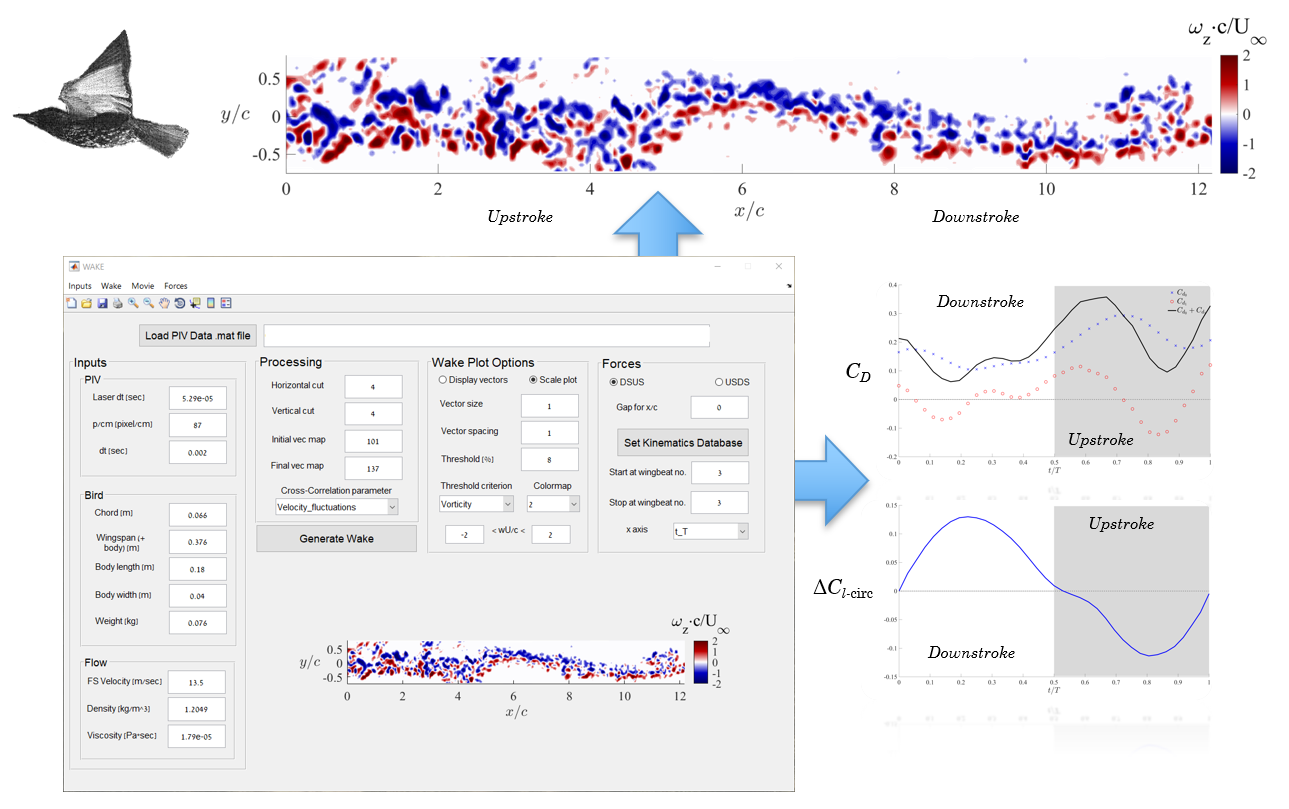
\includegraphics[width=\textwidth]{WAKE-GUI-Overview}
	\label{fig:WAKE-GUI-Overview}
\end{figure}	

\newpage

\tableofcontents

\newpage


\section{Introduction}\label{Intro}

\href{https://github.com/OpenPIV/WAKE-GUI}{\emph{WAKE-GUI} v1.6} is a collection of Matlab subroutines and GUI for post-processing of time-resolved wake data (velocity vector maps) measured using Particle Image Velocimetry (PIV), and analyzed by OpenPIV (or other) software. 
\emph{WAKE-GUI} accepts the PIV wake data as .mat files extracted from the \href{https://github.com/OpenPIV/openpiv-spatial-analysis-toolbox}{OpenPIV spatial analysis toolbox}.
\emph{WAKE-GUI} allows the user to re-construct a full unsteady wake image from a set of PIV images recorded behind bodies/birds using a cross-correlation algorithm.
The \emph{WAKE-GUI} can also be used for estimation of drag and cumulative circulatory lift forces from the wake data, thus enabling the user to estimate the loads exerted on the body generating the wake. 
To cite this software, please use the following:
Ben-Gida, Hadar; Gurka, Roi; Liberzon, Alex (2020): OpenPIV - WAKE-GUI Matlab Toolbox. \textit{figshare}. Software. \url{https://figshare.com/articles/OpenPIV_-_WAKE-GUI_Matlab_ToolBox/12331007}. The source code is available for download in the following GitHub page: \url{https://github.com/OpenPIV/WAKE-GUI}. Contributions to the current version are more than welcome.

The aim of this document is to deliver a detailed description of the \emph{WAKE-GUI} Matlab Toolbox, along with a tutorial. The PIV data used as an example in the tutorial presented here was extracted from wake measurements behind a freely flying Starling (\textit{Sturnus vulgaris}) in a wind-tunnel \cite{Ben-Gida2013,Stalnov2015,Nafi2020}. 

The next sections will refer to the main parameters in the \emph{WAKE-GUI} software, wake processing elements and characterization features, output files and post-processing of the wake to estimate forces. 

\section{Support}\label{Support}

The \emph{WAKE-GUI} can run on Matlab 2015a-2020a versions (cross-platform support).
The tutorial presented here was executed on Matlab 2020a (64bit Windows 10 OS, PC).


\section{Graphical User Interface (GUI)}\label{GUI}

\subsection{Program execution}
The \emph{WAKE-GUI} program starts in Matlab from the command window, by executing the following:

\begin{lstlisting}
WAKE
\end{lstlisting}

Once executed, the Graphical User Interface (GUI) of the \emph{WAKE-GUI} is opened, as depicted in \Cref{fig:GUI-open_window}.

\begin{figure}[ht!]
	\centering
	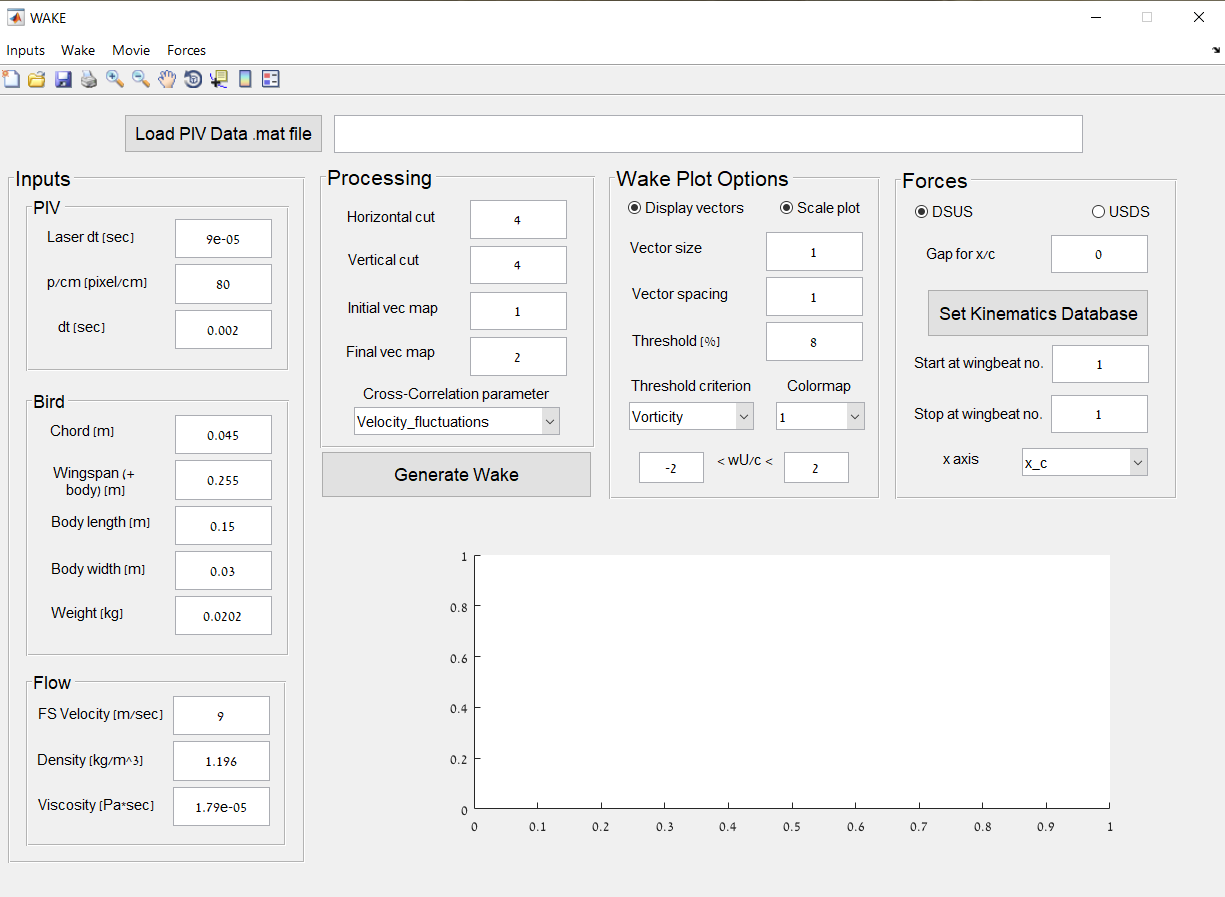
\includegraphics[width=\textwidth]{open_window.png}
	\caption{First window of the \emph{WAKE-GUI}}
	\label{fig:GUI-open_window}
\end{figure}	

\newpage
\subsection{GUI overview}

The \emph{WAKE-GUI} has of several sections (as depicted in \Cref{fig:GUI-sections}):
\begin{itemize}
\item {\color{red}\textbf{Upper menu bar}}: consists of four drop-down menus (``Inputs'', ``Wake'', ``Movie'' and ``Forces''), each has several selectable options that will be explained later in this tutorial.
\item {\color{cyan}\textbf{Editor menu}}: consists of several tools for editing the GUI objects.
\item {\color{blue}\textbf{PIV Data .mat file path}}: placed on the upper middle GUI region and represent the current .mat file path loaded in the GUI (by using the ``Load PIV Data .mat file'' button) for the wake post analysis. This .mat file consists of the PIV velocity vector maps, in a format exported by the \href{https://github.com/OpenPIV/openpiv-spatial-analysis-toolbox}{OpenPIV spatial analysis toolbox}.
\item {\color{brown}\textbf{``Inputs''}}: includes input parameters for the wake analysis in terms of the PIV apparatus, bird characteristics and flow conditions.
\item {\color{green}\textbf{``Processing''}}: consists of parameters relevant for generating the complete wake image from the various instantaneous PIV wake images.
\item {\color{magenta}\textbf{``Wake Plot Options''}}: includes plotting parameters for controlling the presentation of the complete wake image, shown in the lower GUI region.
\item {\color{orange}\textbf{``Forces''}}: includes parameters relevant for the estimation of forces from the wake.
\item {\color{black}\textbf{Wake figure region}}: placed on the bottom GUI region, where the wake image is generated by the GUI.
\end{itemize}

\begin{figure}[ht!]
	\centering
	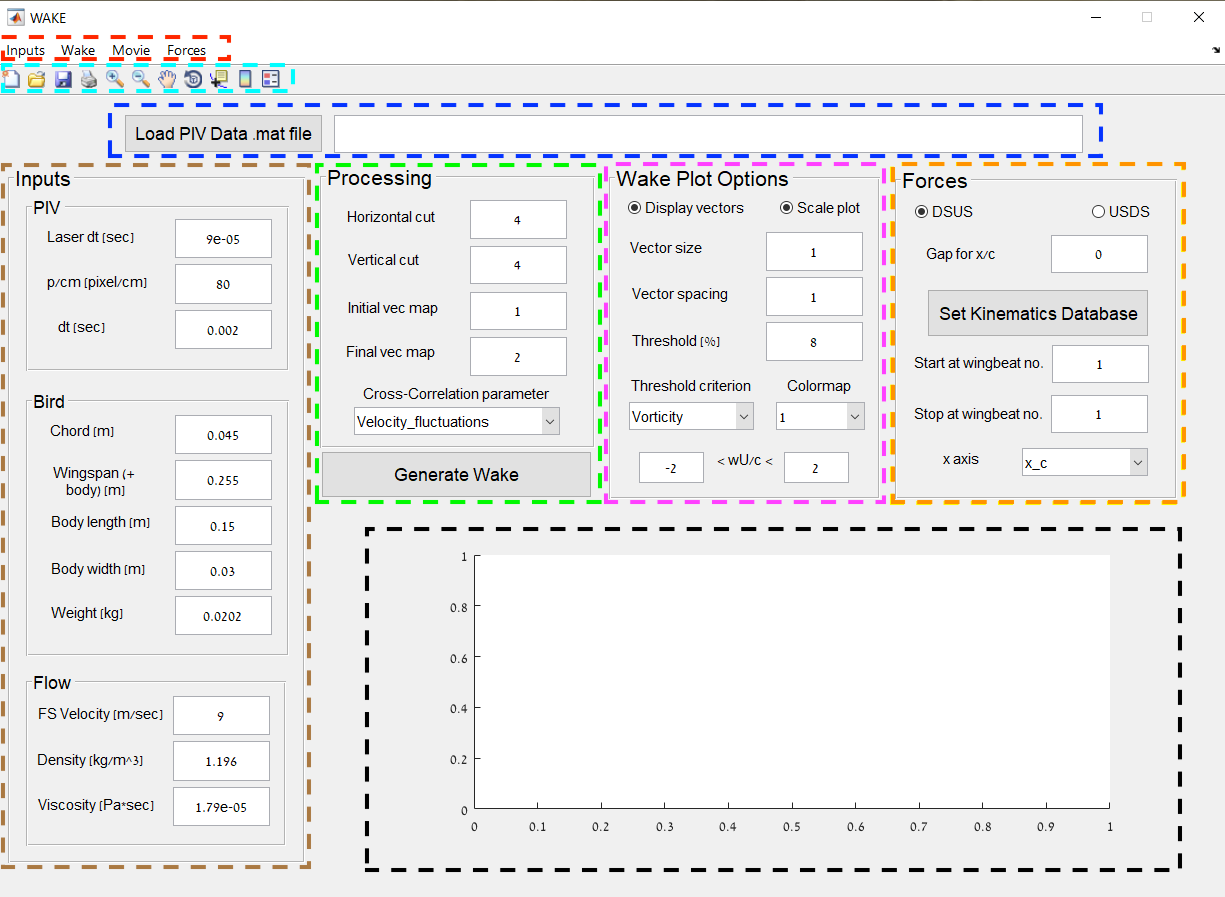
\includegraphics[width=\textwidth]{‏‏open_window_marked_regions}
	\caption{\emph{WAKE-GUI} sections}
	\label{fig:GUI-sections}
\end{figure}	

	

\subsection{Load PIV wake data}

The first step is to load the PIV velocity vector maps as a .mat file format. 
Such .mat file is available by exporting PIV velocity vector maps from the \href{https://github.com/OpenPIV/openpiv-spatial-analysis-toolbox}{OpenPIV spatial analysis toolbox} 
For more information on the export process and the parameters exist in the exported .mat file that is required as an input for the \emph{WAKE-GUI}, the reader is referred to the following \href{https://github.com/OpenPIV/openpiv-spatial-analysis-toolbox/blob/master/docs/tutorial.rst}{webpage tutorial}.
The procedure, in short, is as follows: in the OpenPIV spatial analysis toolbox, on the top left menu bar, under the drop-down menu ``File'', choose one of the load options for the PIV velocity vector maps. Once loaded, export the velocity vector maps by choosing the ``Export to MAT file'' option (under the drop-down menu ``File'').

To load the .mat file in the \emph{WAKE-GUI}, click the ``Load PIV Data .mat file'' button located on the top left region of the GUI, within the PIV Data .mat file path section (see \Cref{fig:GUI-sections}). 
Once clicked, an explorer window will open (``\textit{select the flow data .mat file}''), from which the user can choose the .mat file containing the PIV velocity vector maps (see \Cref{fig:GUI-select_mat_file}). 
In this tutorial, we will choose a .mat file entitled ``\textit{Starling\_2011\_wake\_data.mat}'', which contains velocity vector maps measured in the wake behind a freely flying Starling (\textit{Sturnus vulgaris}) in a wind tunnel. 
The wake data shown here corresponds to four flapping flight wingbeats performed consecutively by the bird. 
Each wingbeat is composed of two phases: a downstroke phase, followed by an upstroke phase; with transition in between.

\begin{figure}[ht!]
	\centering
	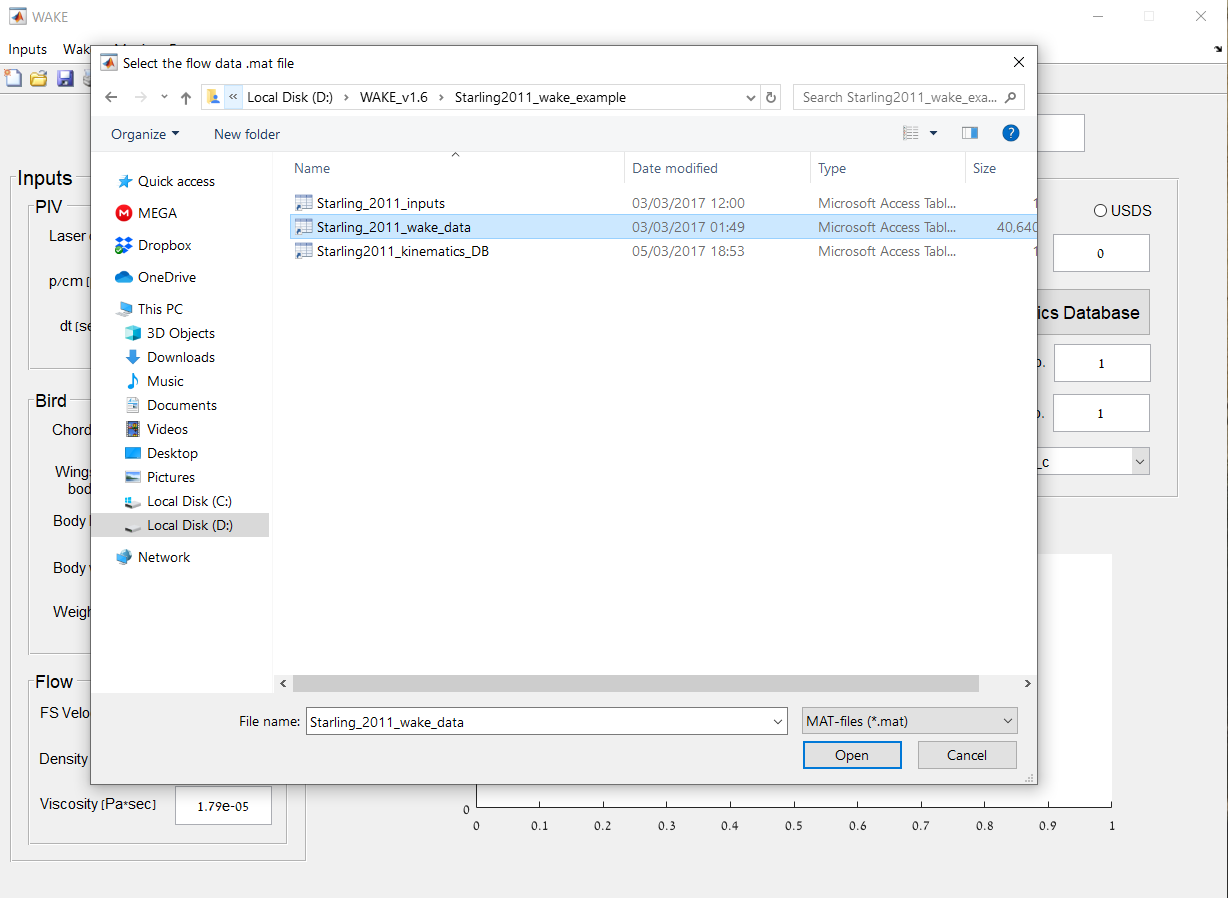
\includegraphics[width=\textwidth]{explorer_window_wake_data.png}
	\caption{Explorer window for selecting the PIV velocity vecotr maps as .mat file}
	\label{fig:GUI-select_mat_file}
\end{figure}


\subsection{Load epxerimental inputs data}
On the top left menu bar, under the drop-down menu ``Inputs'', the option ``Load inputs'' is available (see \Cref{fig:GUI-Inputs-drop-down-menu}), either this option or its shortcut Ctrl+L opens a window where the user can select the experimental inputs data file (.mat format) to be loaded (see \Cref{fig:GUI-Select-inputs-mat-file}).
In this tutorial, we will choose a .mat file entitled ``\textit{Starling\_2011\_inputs.mat}'', which contains the required experimental inputs for analyzing the wake measured behind the bird.
The inputs data .mat file includes information regarding all the parameters within the ``Inputs'' section in the GUI.  The inputs data .mat file can be exported from the GUI by editing the various parameters within the GUI's ``Inupts'' section in the GUI, and then on the top left menu bar, under the drop-down menu ``Inputs'', click the option ``Save inputs'' (see \Cref{fig:GUI-Inputs-drop-down-menu}). 
Either this option or its shortcut Ctrl+I will open a window where the user can export the experimental input data file as a .mat file.

\newpage
\begin{figure}[ht!]
	\centering
	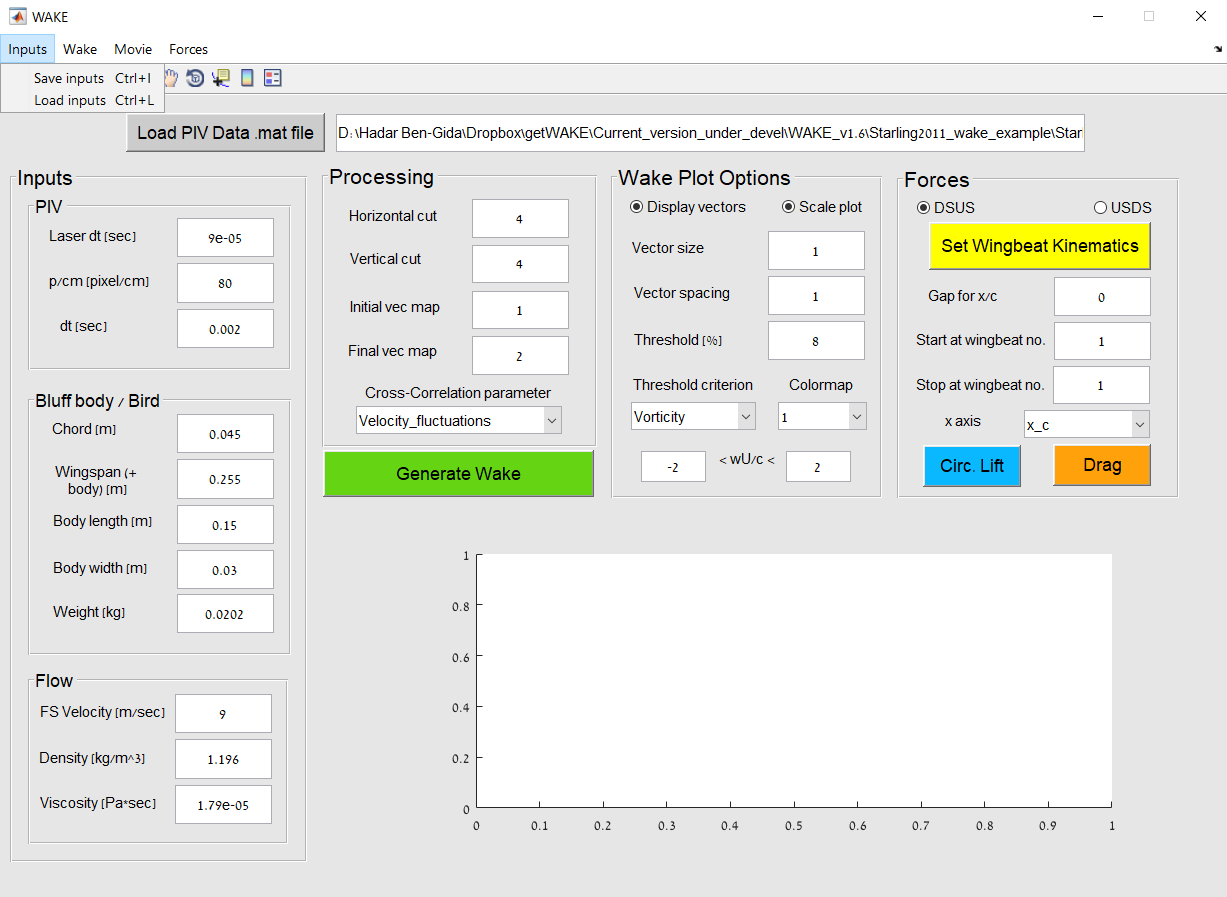
\includegraphics[width=0.9\textwidth]{Inputs-drop-down-menu}
	\caption{Inputs drop-down menu}
	\label{fig:GUI-Inputs-drop-down-menu}
\end{figure}

\begin{figure}[ht!]
	\centering
	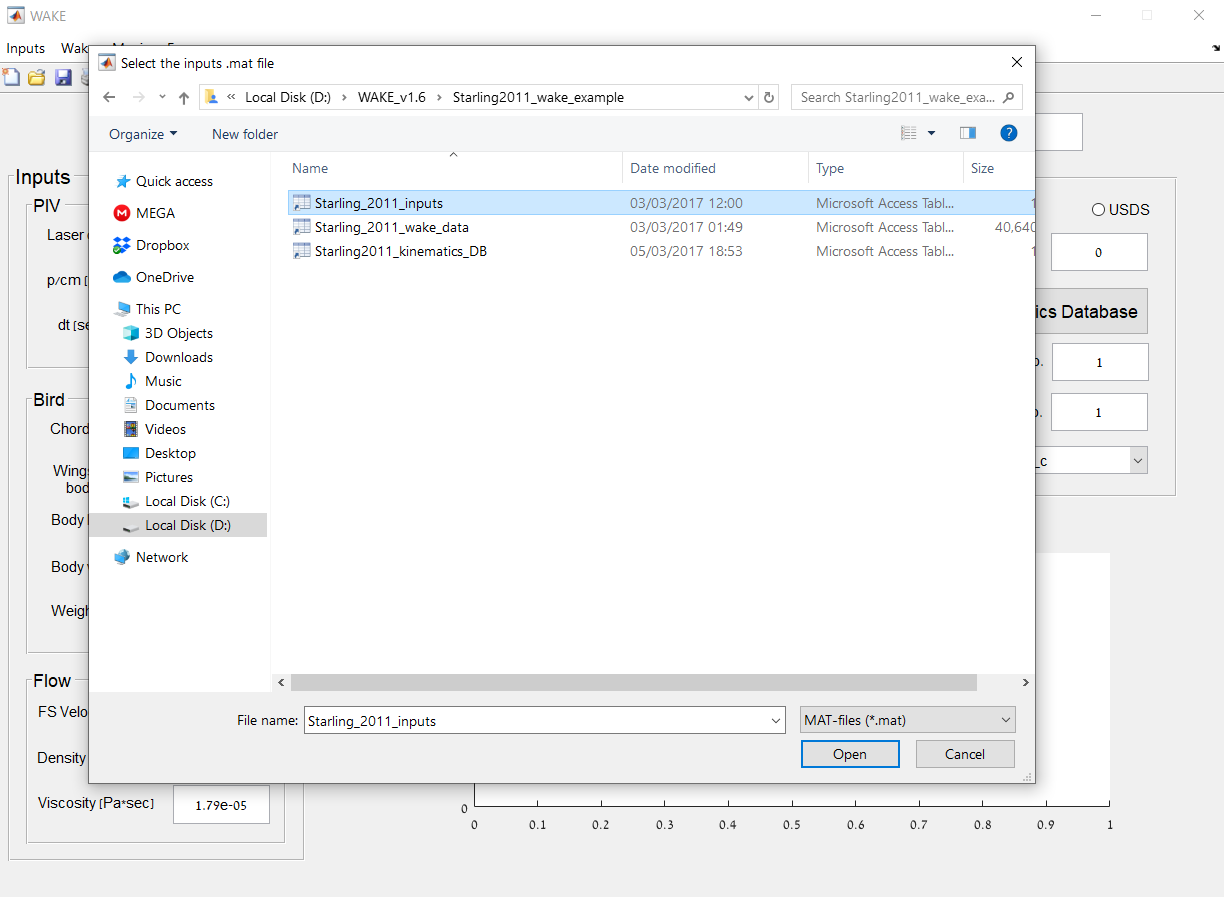
\includegraphics[width=0.9\textwidth]{select-inputs-mat-file}
	\caption{Explorer window for selecting the experimental input data .mat file}
	\label{fig:GUI-Select-inputs-mat-file}
\end{figure}

\newpage
The parameters listed in the GUI's ``Inputs'' section and included in the experimental inputs data .mat file are as follows:
\begin{itemize}
	\item \textbf{Laser dt [sec]}: time difference between the PIV laser's two pulses used to obtain one PIV velocity map from a pair of PIV images in [sec]. 
	\item \textbf{p/cm [pixel/cm]}: pixel-to-centimeter scaling ratio of the PIV velocity maps.
	\item \textbf{dt [sec]}: time difference between two consecutive PIV velocity maps in [sec].
	\item \textbf{Chord [m]}: bird's reference chord length in [m].
	\item \textbf{Wingspan (+ body) [m]}: bird's wingspan length, including the width of the body in [m].
	\item \textbf{Body length [m]}: streamwise length of the bird's body in [m].
	\item \textbf{Body width [m]}: lateral length (width) of the bird's body in [m].
	\item \textbf{Weight [kg]}: bird's weight in [kg].
	\item \textbf{FS Velocity [m/sec]}: Freestream velocity in [m/sec].
	\item \textbf{Density [kg/$\mathrm{m^3}$]}: fluid density in [$\mathrm{kg/m^3}$].
	\item \textbf{Viscosity [kg]}: fluid dynamic viscosity in [$\mathrm{Pa\cdot sec}$].
\end{itemize}


\subsection{Load kinematics database}\label{KIN-DB}

The kinematics database of the bird's wingbeats can be loaded by clicking the ``Set Kinematics Database'' button in the right side of the GUI, within the ``Forces'' section (see \Cref{fig:GUI-set-kinematics-database}). 

\begin{figure}[ht!]
	\centering
	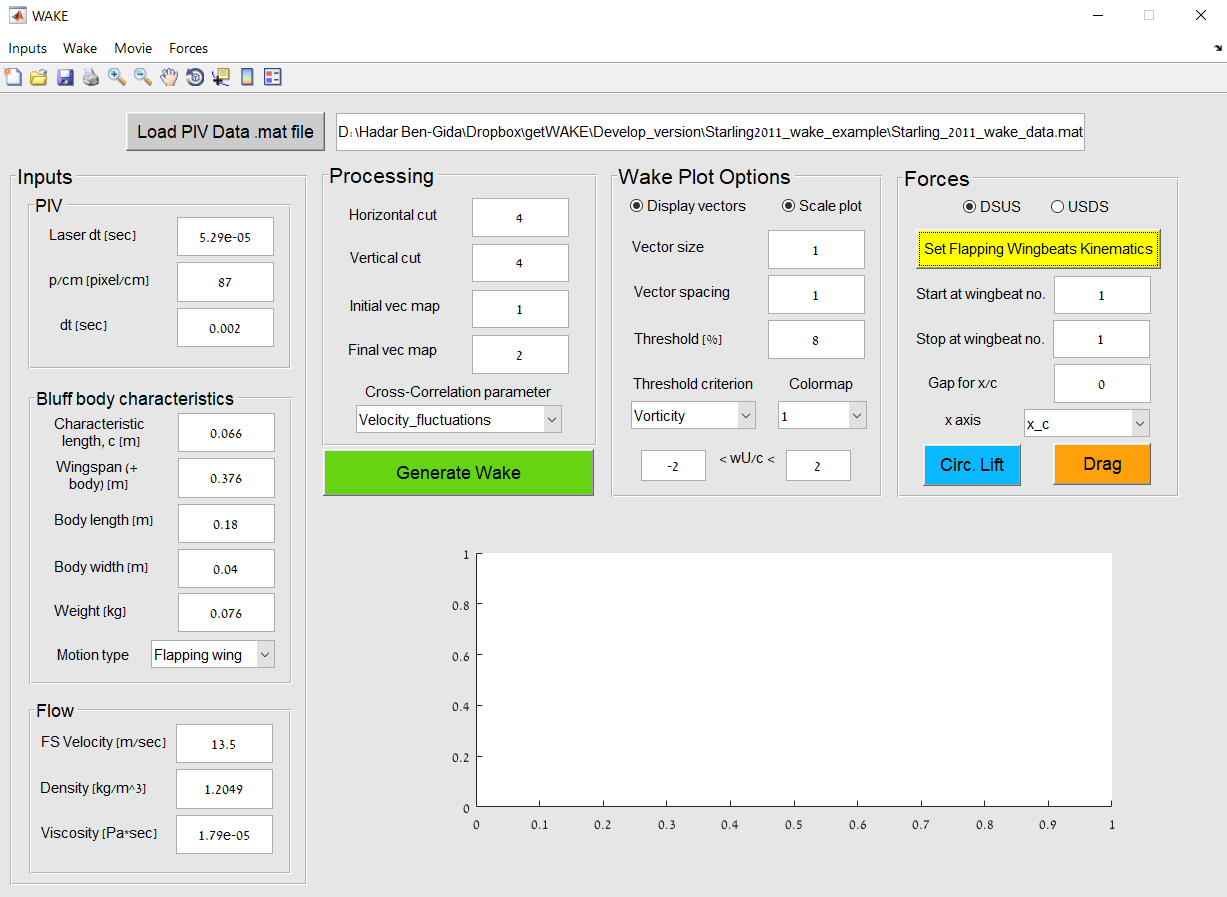
\includegraphics[width=0.71\textwidth]{set-kinematics-database}
	\caption{Set kinematics database button}
	\label{fig:GUI-set-kinematics-database}
\end{figure}

\newpage
This action will open the ``Set Kinematics Info'' window (see \Cref{fig:GUI-kinematics-database-window}), in which the user can edit, load, export and save the kinematics information of the bird in terms of the downstroke, transition and upstroke phases.
Each row in the database correspond to a certain wingbeat in the bird's flight. 
The numbers entered underneath each column (downstroke | transition | upstroke) corresponds to the PIV velocity vector map number in the wake data lodaed to the \emph{WAKE-GUI} that correlates with the specific flight phase.

\begin{figure}[ht!]
	\centering
	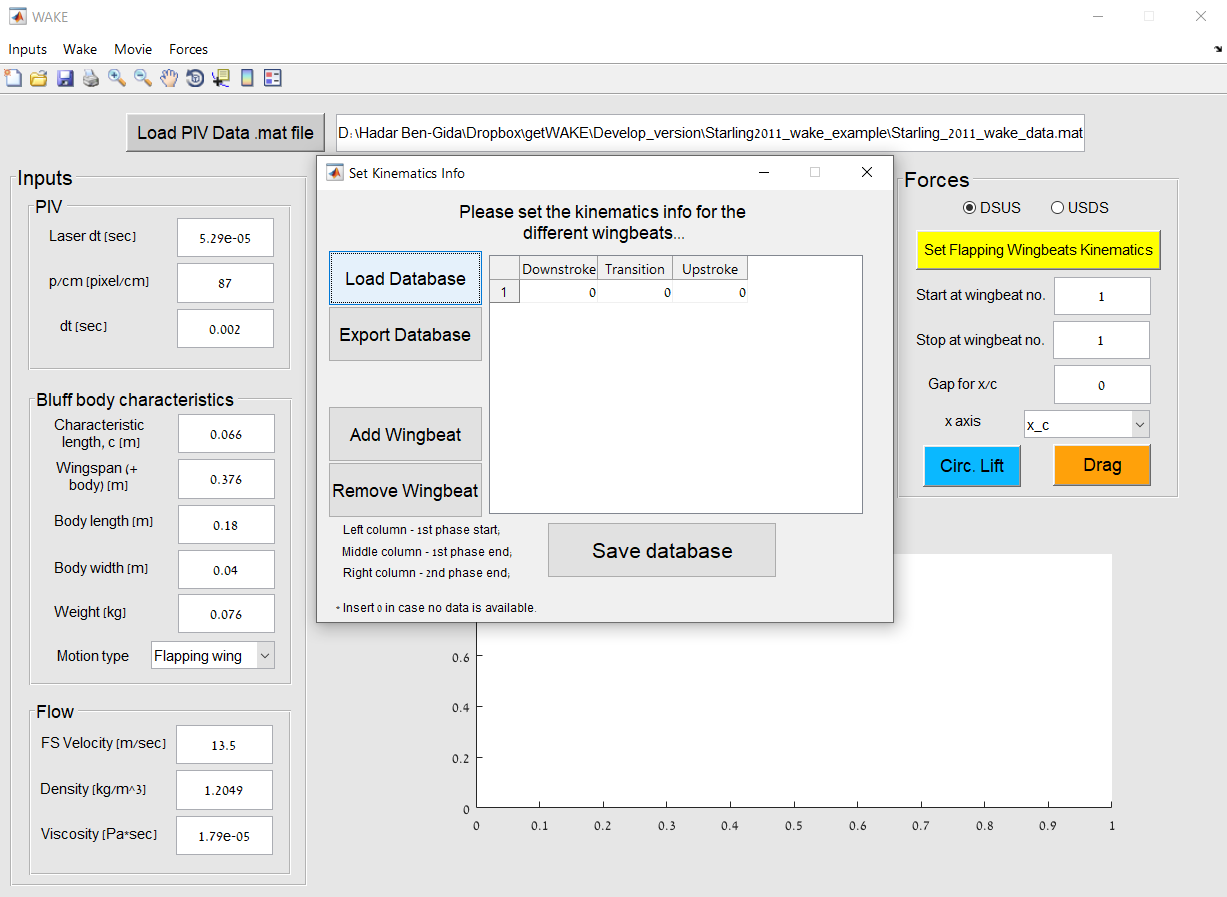
\includegraphics[width=\textwidth]{kinematics-database-window}
	\caption{Set Kinematics information window}
	\label{fig:GUI-kinematics-database-window}
\end{figure}

For example, assume we loaded 175 PIV vector maps describing the bird's wake (as a .mat file, by clicking the ``Load PIV Data .mat file'' button in the GUI), where wake image no. 12-58 correlate with the first wingbeat, wake image no. 58-101 correlate with a second consecutive wingbeat, wake image no. 101-137 correlate with a third consecutive wingbeat and wake image no. 137-174 correlate with a fourth consecutive wingbeat. For the first wingbeat, wake image no. 12 marks the start of its downstroke phase, wake image no. 34 marks the end of the downstroke phase and wake image no. 58 marks the end of the upstroke phase. For the second wingbeat, wake image no. 58 marks the start of its downstroke phase, wake image no. 78 marks the end of the downstroke phase and wake image no. 101 marks the end of the upstroke phase. For the third wingbeat, wake image no. 101 marks the start of its downstroke phase, wake image no. 119 marks the end of the downstroke phase and wake image no. 137 marks the end of the upstroke phase. For the fourth wingbeat, wake image no. 137 marks the start of its downstroke phase, wake image no. 155 marks the end of the downstroke phase and wake image no. 174 marks the end of the upstroke phase.
Therefore, one has to edit the kinematics database table as depicted in \Cref{fig:GUI-Kinematics-db-filled}; adding/removing wingbeats in the table can be done by clicking the ``Add Wingbeat''/``Remove Wingbeat'' button. 
Here, the kinematics database presented in \Cref{fig:GUI-Kinematics-db-filled} corresponds to four consecutive flapping flight wingbeats of the Starling. 

After finish editing the kinematics databse table, the user can save the database in the \emph{WAKE-GUI} workspace for further analysis, by clicking the ``Save database'' button in the ``Set Kinematics Info'' window. 
The user can also export the kinematics database as a .mat file for future usage by clicking the ``Export Databse'' button in the ``Set Kinematics Info'' window. 
This .mat file format can be re-loaded to the \emph{WAKE-GUI} workspace by clicking the ``Load Database'' button in the ``Set Kinematics Info'' window.
Please be sure to click the ``Save database'' button after finish editing the kinematics database and before exiting the ``Set Kinematics Info'' window, so the database will be available in the \emph{WAKE-GUI} workspace.


\begin{figure}[ht!]
	\centering
	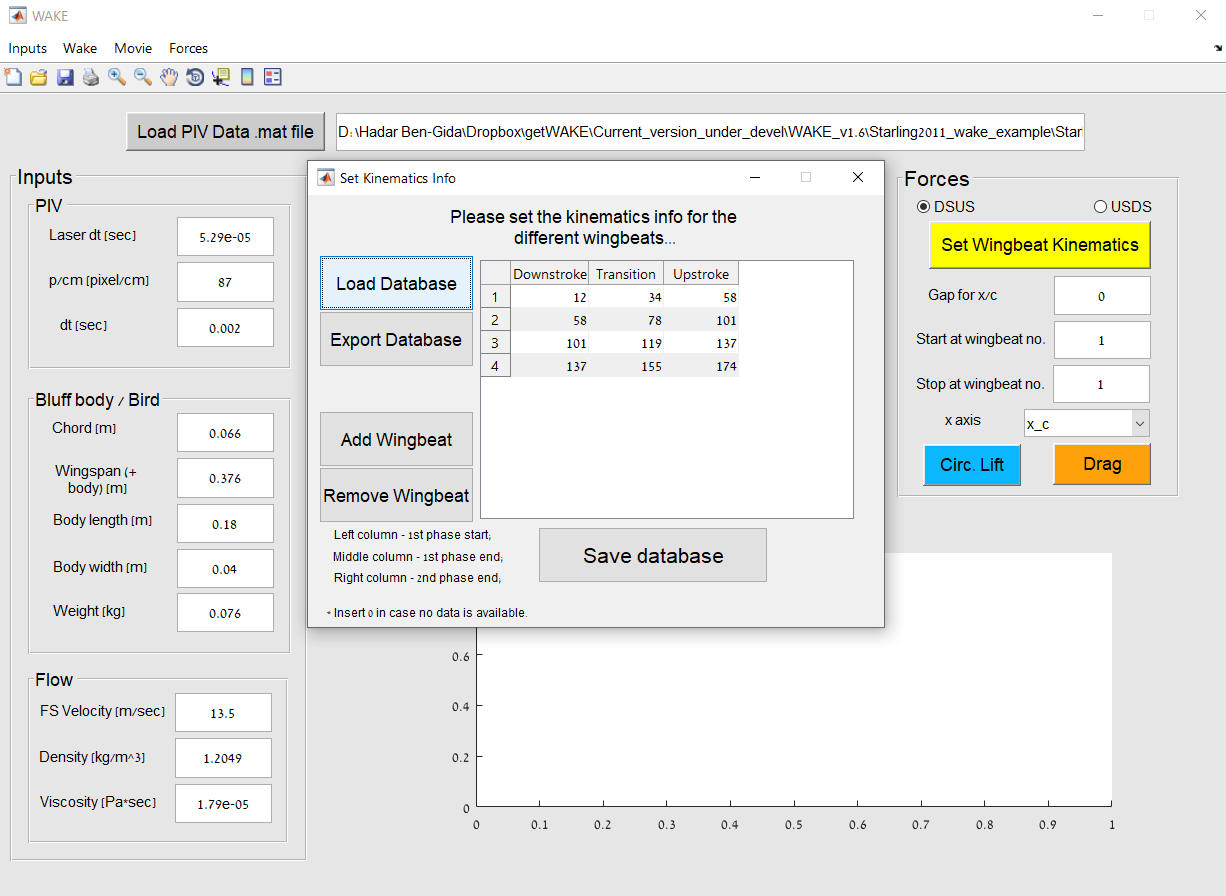
\includegraphics[width=\textwidth]{Kinematics-db-filled}
	\caption{Kinematics database table filled for four consecutive flapping flight wingbeats of a Starling}
	\label{fig:GUI-Kinematics-db-filled}
\end{figure}



\newpage
\subsection{Processing the PIV wake data}
After importing the PIV wake data, experimental inputs data and kinematics DB (database), one can analyze a sequence of instantaneous wake images (time-resolved PIV velocity maps) and compose a complete wake image, depicting the flow structures as they evolve downstream the source.
In the ``Processing'' section, we enter the following parameters for processing the wake (see \Cref{fig:GUI-Wake-processing-parameters}):
\begin{itemize}
	\item \textbf{Horizontal cut}: number of vector columns to remove from both the left and rights edges of each instantaneous PIV velocity map, before processing the wake images in the sequence (\textit{default} value is 4).
	\item \textbf{Vertical cut}: number of vector columns to remove from both the top and bottom edges of each instantaneous PIV velocity map, before processing the wake images in the sequence (\textit{default} value is 4).
	\item \textbf{Initial vec map}: initial PIV wake image number in the wake images sequence from the loaded wake data .mat file (\textit{default} value is 1).
	\item \textbf{Final vec map}: final PIV wake image number in the wake images sequence from the loaded wake data .mat file (\textit{default} value is 1).
	\item \textbf{Cross-Correlation parameter}: menu bar for defining the flow parameter according to which the cross-correlation algorithm will perform for each pair of consecutive wake images to construct the complete wake image. Two flow parameters are available for the cross-correlation algorithm:  ``\textit{velocity fluctuations}'' or ``\textit{velocity}''; i.e., ($u^\prime, v^\prime$) or ($u,v$). (\textit{default} value is ``\textit{velocity fluctuations}'').
\end{itemize}
  
\begin{figure}[ht!]
 	\centering
 	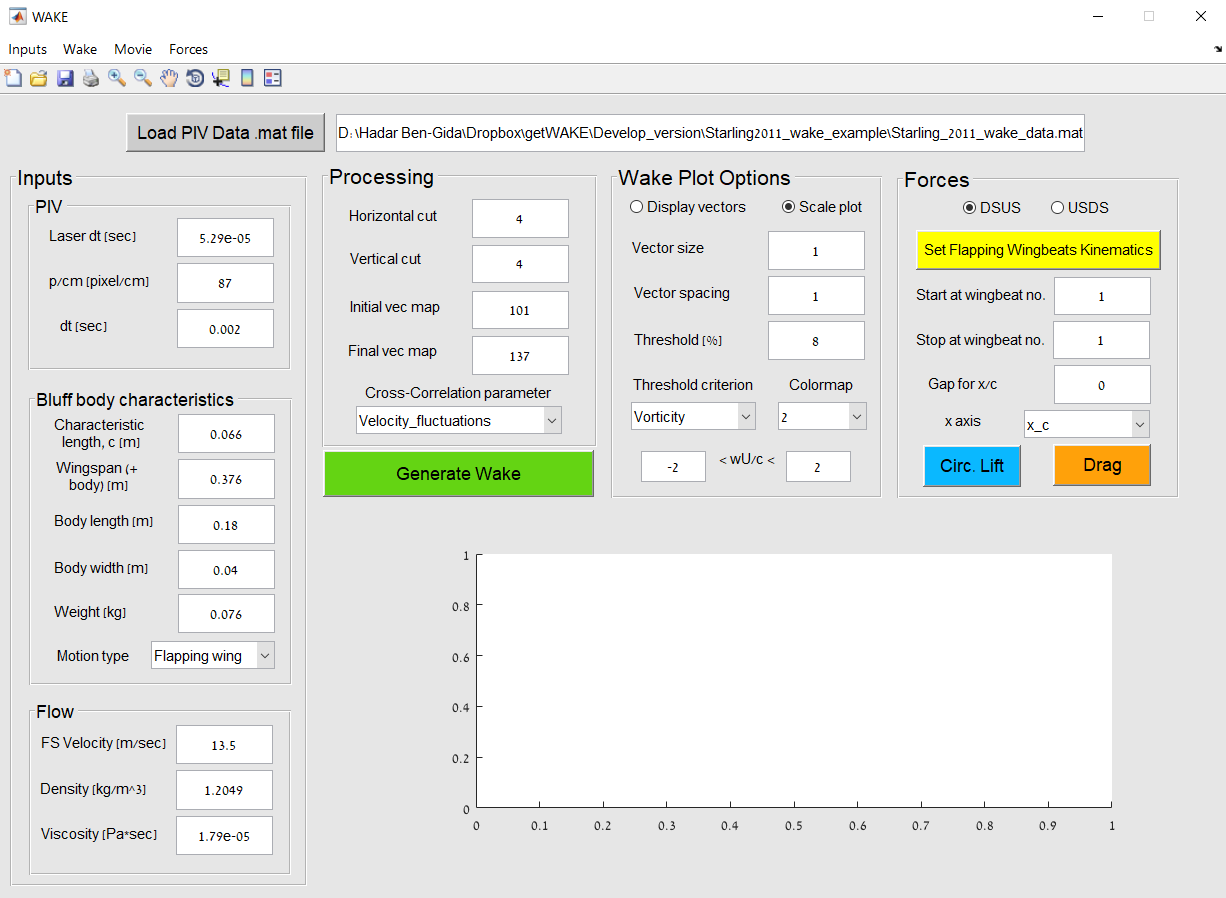
\includegraphics[width=0.79\textwidth]{Wake-processing-parameters}
 	\caption{Parameters for processing the PIV wake images}
 	\label{fig:GUI-Wake-processing-parameters}
\end{figure}

  After defining the various parameters above, the user can now generate the complete wake image. This is done by pressing the ``Generate Wake' push button. Pressing this button will perform the main computation of generating the complete wake from the sequence of wake images chosen by the user and according to the selected processing parameters. The progress of the computation process is shown in a new open window (see \Cref{fig:GUI-generating-wake-progress}). When the computation completed the complete wake will be plotted in the ``Wake figure region'' (see \Cref{fig:GUI-wake-generated}).  
  
\begin{figure}[ht!]
	\centering
	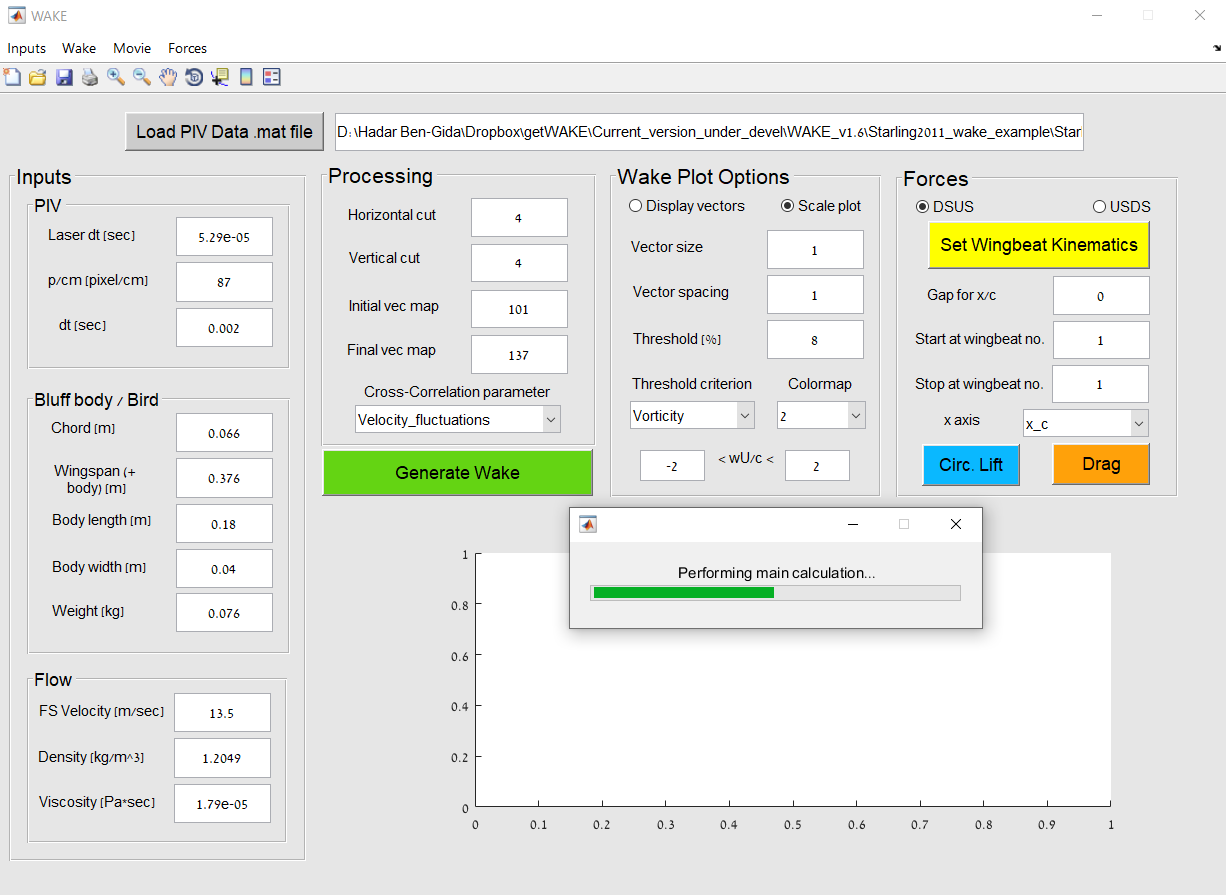
\includegraphics[width=0.77\textwidth]{Generating_Wake_processing}
	\caption{Window showing the progress of the complete wake computation}
	\label{fig:GUI-generating-wake-progress}
\end{figure}
  
\begin{figure}[ht!]
	\centering
	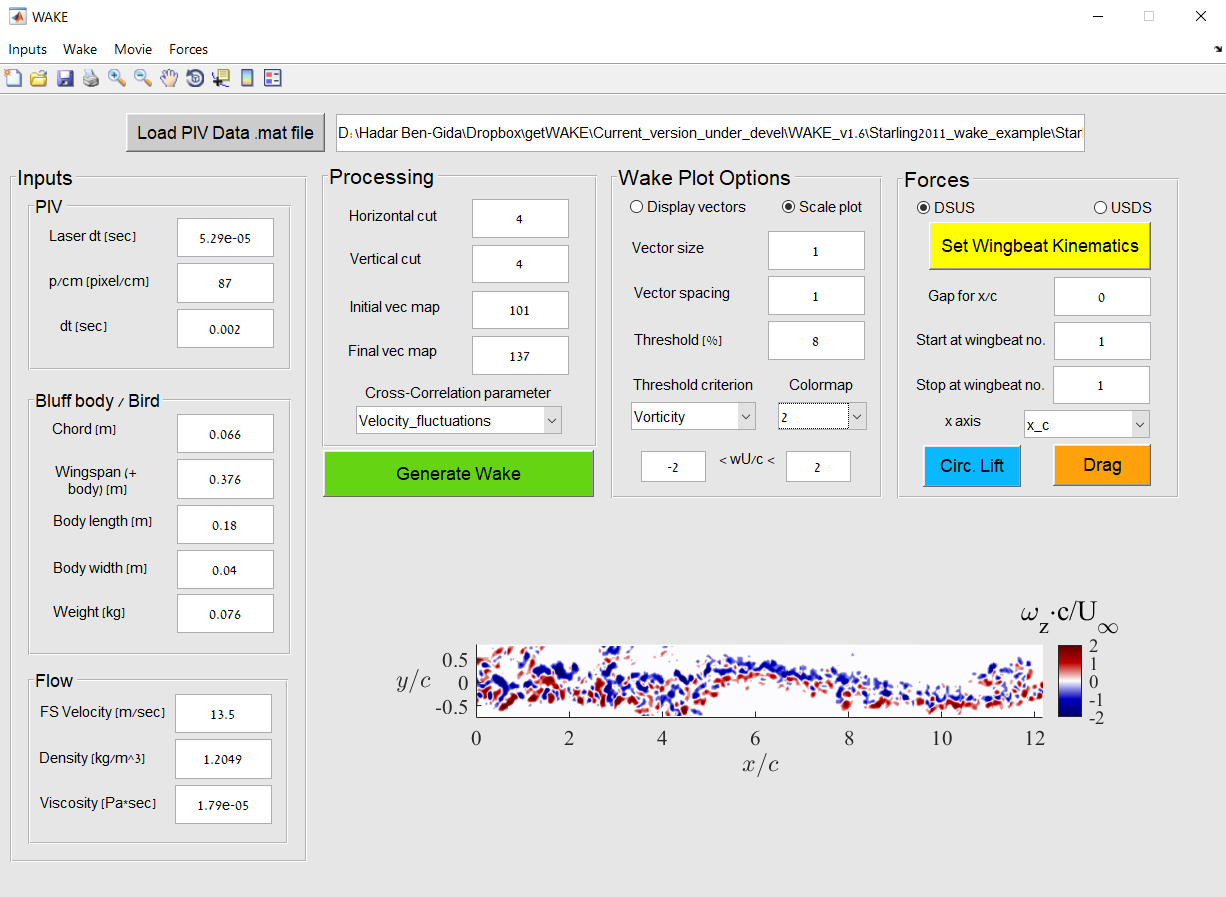
\includegraphics[width=0.77\textwidth]{wake-generated}
	\caption{The complete wake image plotted in the ``Wake figure region''}
	\label{fig:GUI-wake-generated}
\end{figure}
 
 \newpage
 \subsection{Wake plot options}
Once a complete wake image was generated, the user can edit the plot from the ``Wake Plot Options'' section, by using the following parameters (see \Cref{fig:GUI-wake-generated}):
\begin{itemize}
	\item \textbf{Display vectors}: on/off button for plotting the velocity vectors in the complete wake image (\textit{default} status is \textit{on}).
	\item \textbf{Scale plot}: on/off button for equaling the scale of the complete wake image axes (\textit{default} status is \textit{on}).
	\item \textbf{Vector size}: vectors size plotted in the complete wake image (\textit{default} value is 1).
	\item \textbf{Vector spacing}: spacing between the velocity vectors plotted in the complete wake image (\textit{default} value is 1).
	\item \textbf{Threshold}: threshold percentage value [\%] for the vortices in the complete wake image. The vortices visible in the complete wake image will be those with vorticity/swirl (depends on the threshold criterion set by the user) value that exceeds the threshold percentage value from the maximum absolute vorticity/swirl value in the wake image; e.g., assuming the user choose the vorticity as the threshold criterion, if the maximum absolute vorticity in the complete wake image is 5 $\mathrm{sec^{-1}}$ and the threshold vorticity percentage set by the user is 8\%, then, vortices with absolute vorticity value under 0.4 $\mathrm{sec^{-1}}$ will not be shown in the complete wake image (\textit{default} value is 8).
	\item \textbf{Threshold criterion}: the flow quantity according to which a threshold is applied on the complete wake image. Two options are available (\textit{default} parameter is ``\textit{vorticity}''): 
	\begin{itemize}
		\item vorticity - $\frac{\partial v}{\partial x} - \frac{\partial u}{\partial y}$
		\item swirl - $\bm{\mathrm{Im}}\left[ \sqrt{ \frac{1}{4}\left(\frac{\partial u}{\partial x} + \frac{\partial v}{\partial y}\right)^2+ \left(\frac{\partial u}{\partial y} \frac{\partial v}{\partial x} \right) - \left(\frac{\partial u}{\partial x} \frac{\partial v}{\partial y} \right)}  \right]$ 
	\end{itemize}
	\item \textbf{Colormap}: color map for the complete wake image. Five color maps are available in total (\textit{default} value is 1).
	\item \bm{$< \omega U/c <$}: range of normalized vorticity values in the color bar of the plotted wake image (\textit{default} values are -2 to 2).
\end{itemize}
Please note that any editing done in the ``Wake Plot Options'' section will immediately affect the complete wake image, re-plotting it.

On the top left menu bar, under ``Wake'', several more options exist.
The user can open the wake image in a new figure window for better visualization and inspection of the flow structures in the wake by clicking the option ``Open wake in a new window'' or using the shortcut Ctrl+P (see \Cref{fig:GUI-wake-menubar}).
The complete wake image can also be exported as a figure file by clicking the option ``Save wake plot'' or using the shortcut Ctrl+S (see \Cref{fig:GUI-wake-menubar}).
Vorticity values computed in the complete wake image can be exported as a .mat. file for further analysis by clicking the option ``Save wake vorticity map'' or using the shortcut Ctrl+V (see \Cref{fig:GUI-wake-menubar}).
  
  \newpage
 \begin{figure}[ht!]
 	\centering
 	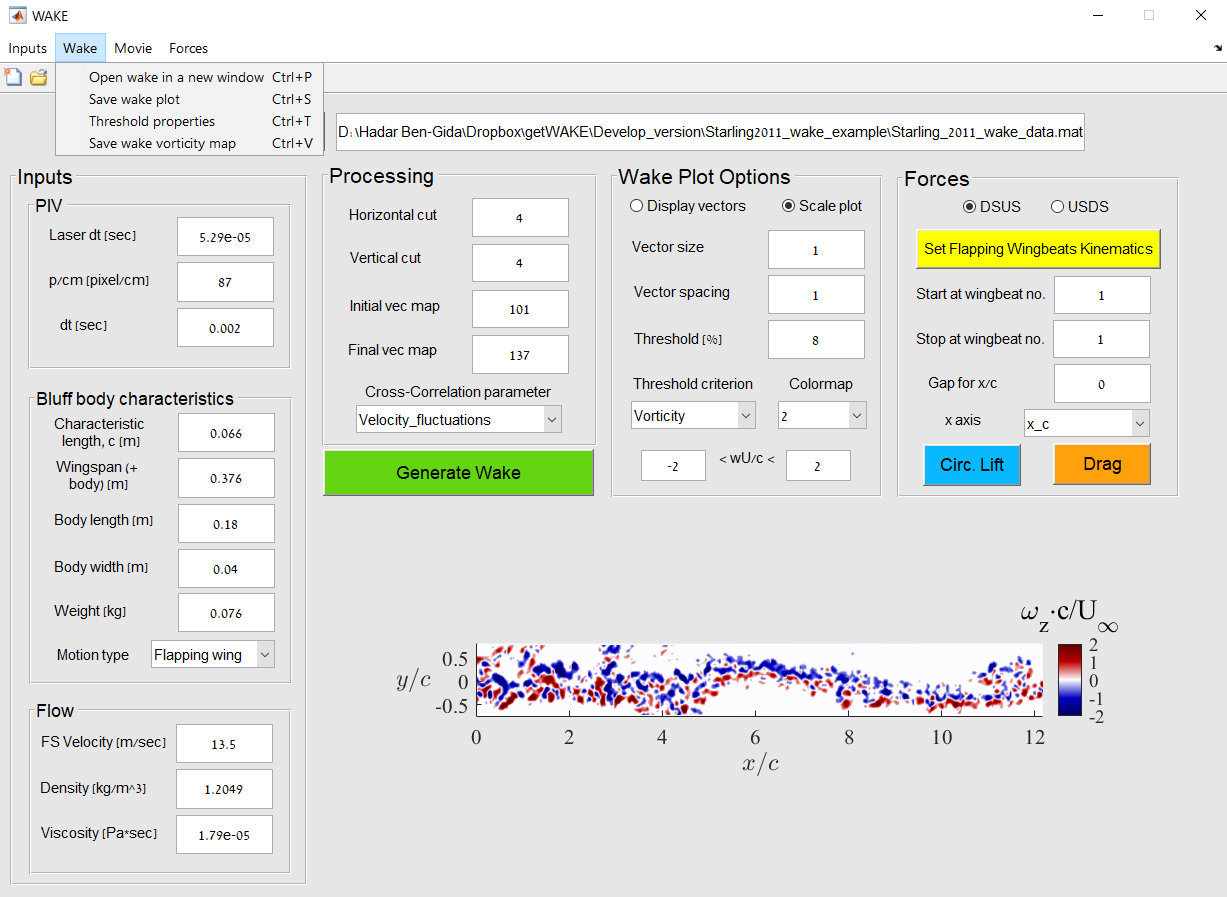
\includegraphics[width=0.87\textwidth]{Wake-menuber-options}
 	\caption{Options in the ``Wake'' menu bar}
 	\label{fig:GUI-wake-menubar}
 \end{figure}

The user can edit the properties of the threshold utilized by clicking the option ``Threshold properties'' or using the shortcut Ctrl+T (see \Cref{fig:GUI-wake-menubar}). 
This will open a new window entitled ``Threshold properties'' (see \Cref{fig:GUI-Wake-threshold-properties}). 

\begin{figure}[ht!]
	\centering
	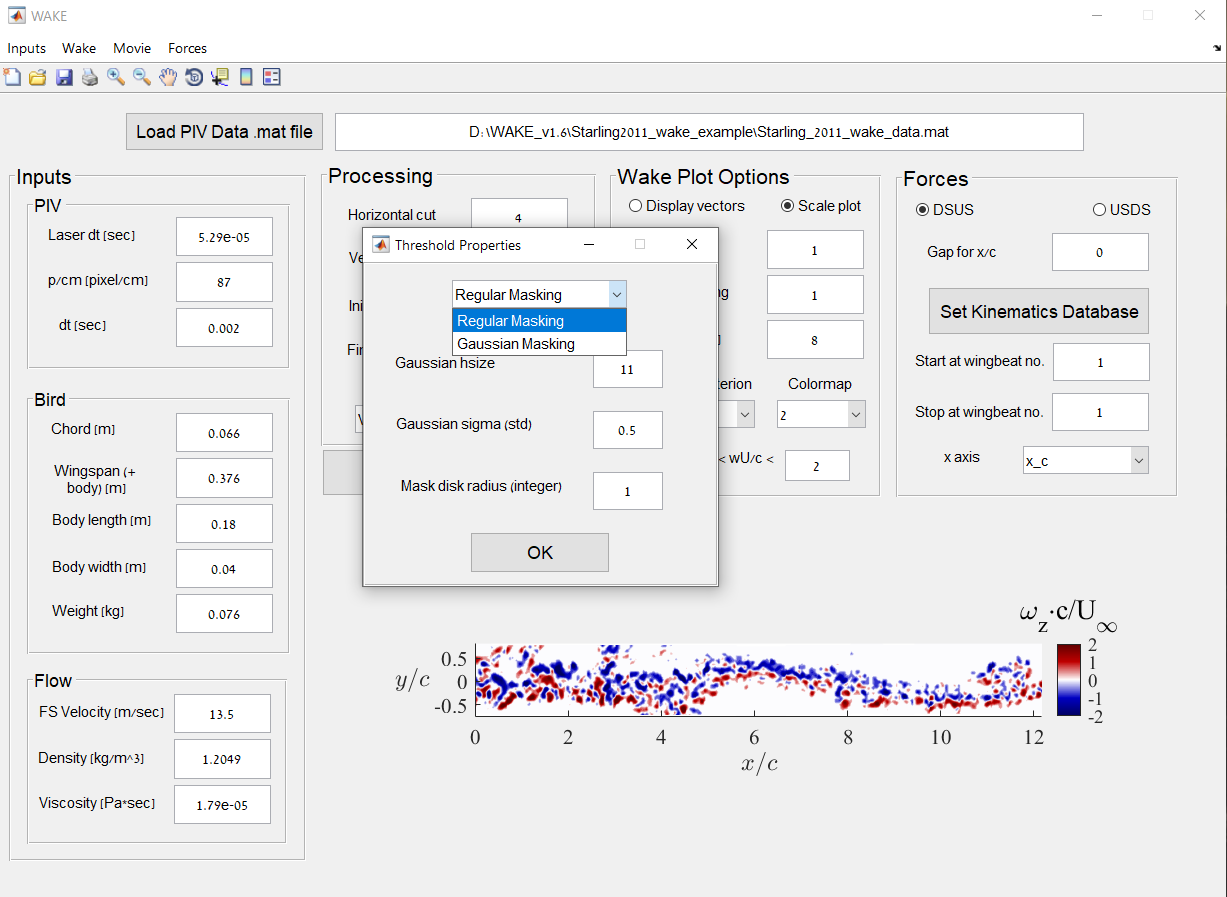
\includegraphics[width=0.87\textwidth]{Wake-threshold-properties}
	\caption{Wake threshold properties}
	\label{fig:GUI-Wake-threshold-properties}
\end{figure}

Two masking options exist for the threshold to be applied on the complete wake image (\textit{default} option is ``\textit{Regular Masking}''):
\begin{itemize}
	\item ``Regular Masking'' - applies the threshold directly on the wake data array with no smoothing.
	\item ``Gaussian Masking'' - applies a 2D rotationally symmetric Gaussian lowpass filter with size that is indicated in ``Gaussian hsize'' and standard deviation that is indicated in ``Gaussian sigma (std)''. The radius of the masking Gaussian disk is indicated by ``Mask disk radius (integer)'' in terms of array elements.
\end{itemize}
When finished, clicking the ``OK'' button will confirm the changes done.

The user can also export a movie of the PIV wake data sequence chosen in the ``Processing'' section. 
On the top left menu bar, under the drop-down menu ``Movie'', the option ``Save movie'' is available (see \Cref{fig:GUI-Movie-menubar}), either this option or its shortcut Ctrl+M will export a movie of the PIV wake data sequence.
The properties of the exported movie can be determined from the ``Movie properties'' option under the drop-down menu ``Movie''. 
Either this option or its shortcut Ctrl+N will open a new window entitled ``Movie properties'' (see \Cref{fig:GUI-movie-properties}), in which the user can set the frames per second rate in the exported movie.

\begin{figure}[ht!]
	\centering
	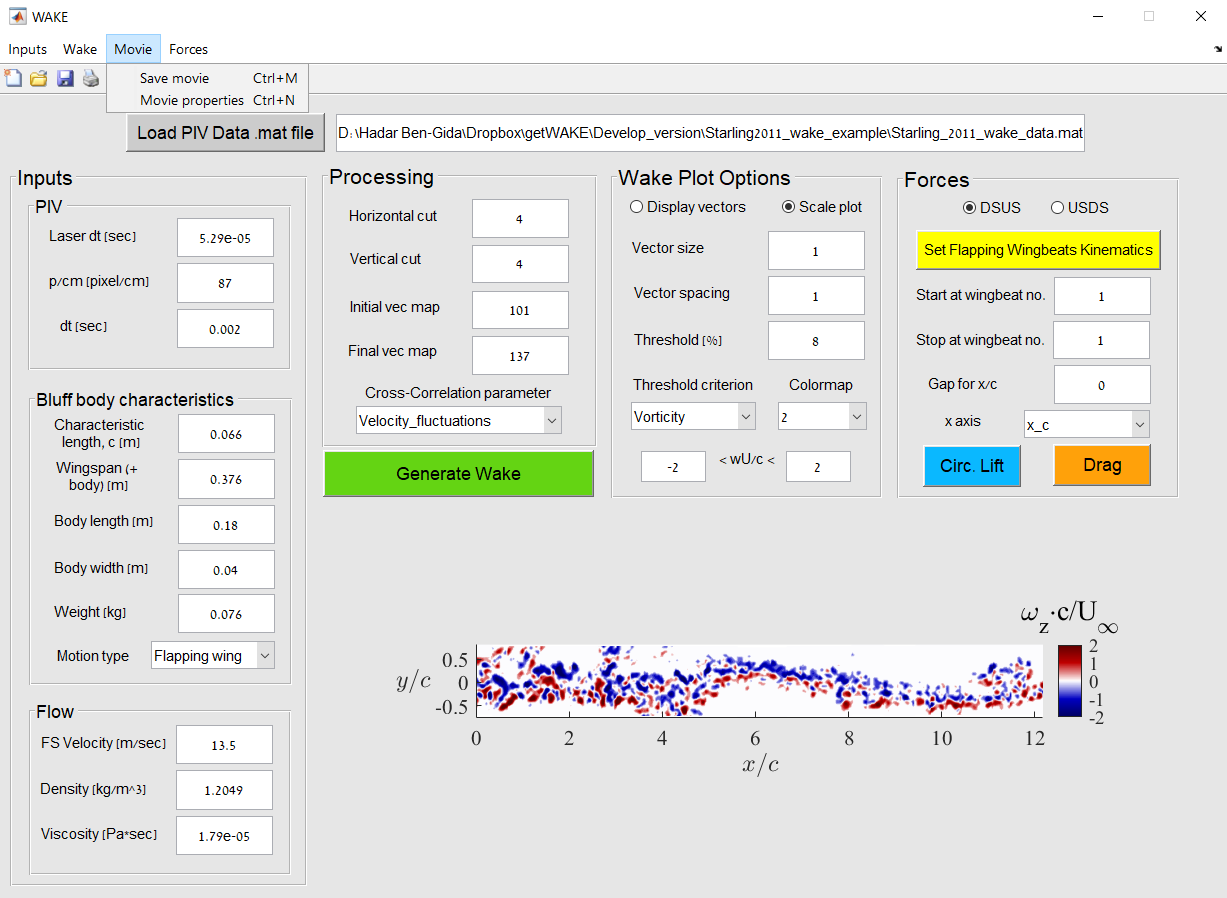
\includegraphics[width=0.9\textwidth]{Movie-menubar}
	\caption{Options in the ``Movie'' menu bar}
	\label{fig:GUI-Movie-menubar}
\end{figure}

\begin{figure}[ht!]
	\centering
	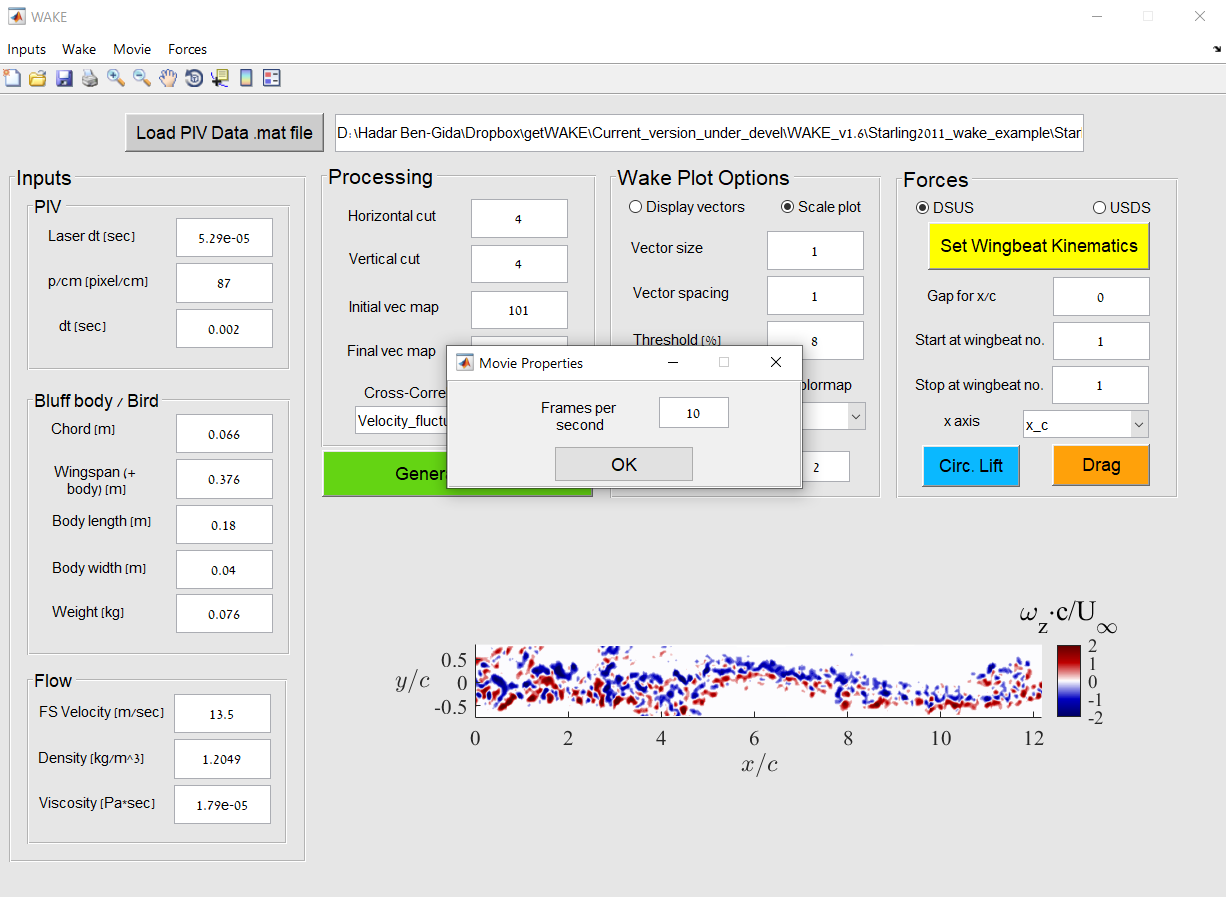
\includegraphics[width=0.86\textwidth]{movie-properties}
	\caption{Movie properties}
	\label{fig:GUI-movie-properties}
\end{figure}

\newpage
\subsection{Forces estimation}\label{forces_estimation}
The user can estimate the variation of drag and cumulative circulatory lift throughout the wake, for various wingbeat cycles, vs. time or streamwise distance ($x/c$). 
To do so, the user first needs to define several parameters in the ``Forces'' section (see \Cref{fig:GUI-Forces-menubar}):
\begin{itemize}
	\item \textbf{DSUS}: on/off button for specifying that the flapping wingbeats are characterized first with a downstroke phase that is followed with an upstroke phase (\textit{default} status is \textit{on}).
	\item \textbf{USDS}: on/off button for specifying that the flapping wingbeats are characterized first with an upstroke phase that is followed with a downstroke phase (\textit{default} status is \textit{off}).
	\item \textbf{Gap for x/c}: setting an artificial normalized streamwise extent shift, after which the forces estimation will be plotted; e.g., if set to 5, the forces plots will not start from $x/c=0$, but from $x/c=5$. This parameter is only applicable for plotting the forces vs. the streamwise distance, $x/c$ (\textit{default} value is 0).
	\item \textbf{Set Kinematics Database}: push button (see \Cref{KIN-DB}); when clicked will open a new window entitled ``Set Kinematics Info'' for setting the kinematics database of the various wingbeats. The phases definition in this database will determine how the forces variation throughout the wake will be presented for the various wingbeat cycles.
	\item \textbf{Start at wingbeat no.}: initial wingbeat no. from which the forces variation plot will start, according to the kinematics database (\textit{default} value is 1).
	\item \textbf{Stop at wingbeat no.}: final wingbeat no. up to which the forces variation will be presented, according to the kinematics database (\textit{default} value is 1).
	\item \textbf{x axis}: define the $x$ axis in the plots of the forces variation throughout the wake. Two options are available (\textit{default} option is ``\textit{x\_c}''):
	\begin{itemize}
		\item ``x\_c'' - plots the forces estimation vs. the normalized streamwise distance of the wake, $x/c$.
		\item ``t\_T'' - plots the forces estimation vs. the normalized time, $t/T$; where $T$ is the wingbeat total time period.
	\end{itemize}
\end{itemize}
Please note, the user can plot the forces variation for multiple wingbeats (``Start at wingbeat no.''<``Final at wingbeat no.'') or for a single wingbeat (``Start at wingbeat no.''=``Final at wingbeat no.''). If choosing to plot the forces variation for multiple wingbeats, the $x$ axis can only be depicted in terms of absolute time, $t$, and not the normalized time, $t/T$; as the time period, $T$, can be different for multiple wingbeats. 


\begin{figure}[ht!]
	\centering
	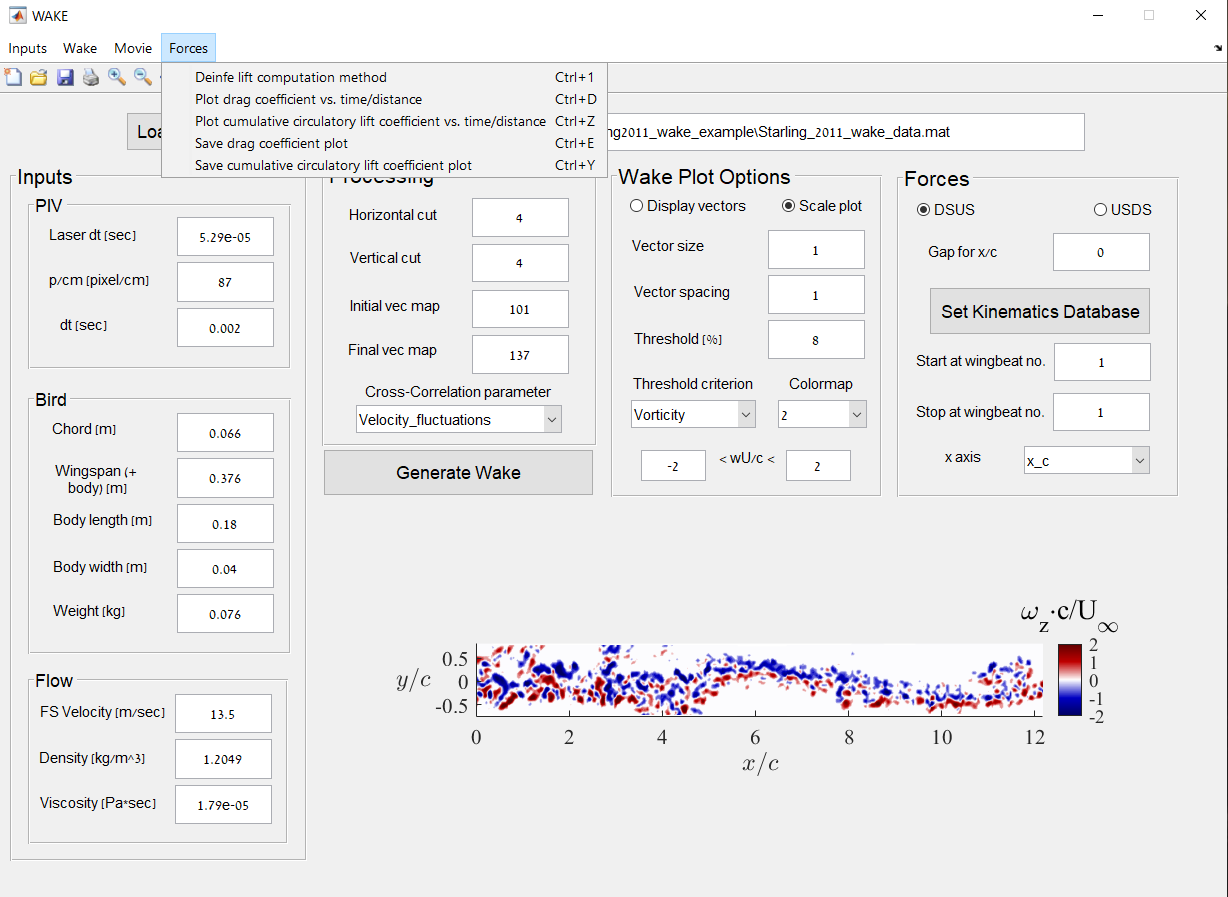
\includegraphics[width=0.77\textwidth]{Forces-menubar}
	\caption{Options in the ``Forces'' menu bar}
	\label{fig:GUI-Forces-menubar}
\end{figure}



Ploting the variation of forces along the wake is available on the top left menu bar, under the drop-down menu ``Forces''. 
The option ``Plot cumulative circulatory lift coefficient vs time/distance'' or its shortcut Ctrl+Z (see \Cref{fig:GUI-Forces-menubar}) will plot the variation in the cirulatory lift coefficient $\Delta C_{l_{circ}}$ vs. time (see \Cref{fig:GUI-dCl-plot}) or $x/c$ (see \Cref{fig:GUI-dCl-plot-vs-x_c}), depending on the ``x axis'' parameter. The option ``Save cumulative circulatory lift coefficient plot'' or its shortcut Ctrl+Y will export the variation in the circulatory lift coefficient as an image file.
\Cref{fig:GUI-dCl-plot-vs-time-4-wingbeats} depicts the time variation of the cumulative circulatory lift coefficient for four consecutive Starling wingbeats.
The option ``Plot drag coefficient vs time/distance'' or its shortcut Ctrl+D (see \Cref{fig:GUI-Forces-menubar}) will plot the drag coefficient $C_d$ vs. time or $x/c$, depending on the ``x axis'' parameter (see \Cref{fig:GUI-drag-plot}). The option ``Save drag coefficient plot'' or its shortcut Ctrl+E will export the drag coefficient figure as an image file.
Please note, the white shaded region in the above plots corresponds to the downstroke phase in the wingbeat, whereas the gray shaded region corresponds to the upstroke phase. $C_{d_0}$ and $C_{d_1}$ are the steady and unsteady components of the drag coefficient, respectively.


\begin{figure}[ht!]
	\centering
	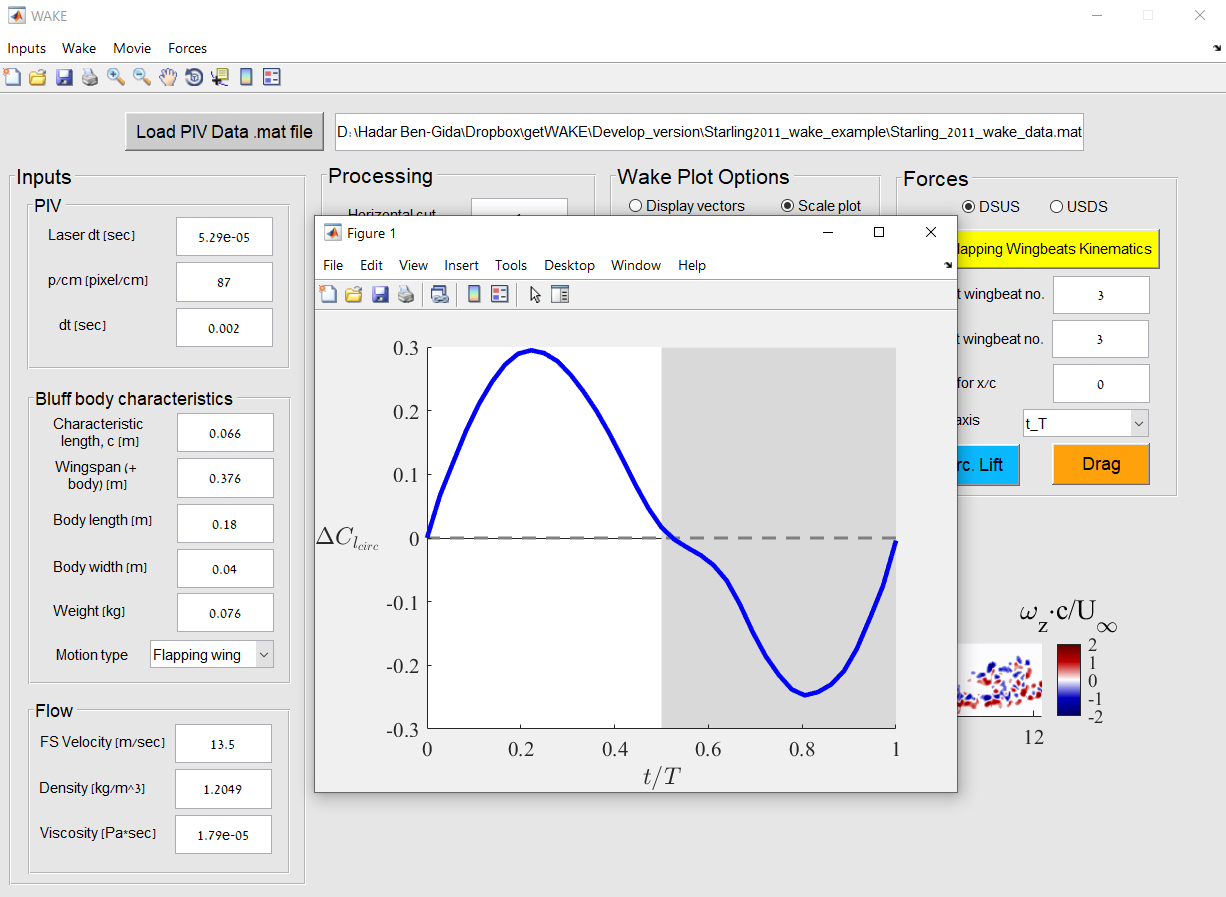
\includegraphics[width=0.79\textwidth]{dCl-plot}
	\caption{Variation of the cumulative circulatory lift coefficient with $t/T$ for the $3^\mathrm{rd}$ Starling's wingbeat}
	\label{fig:GUI-dCl-plot}
\end{figure}

\begin{figure}[ht!]
	\centering
	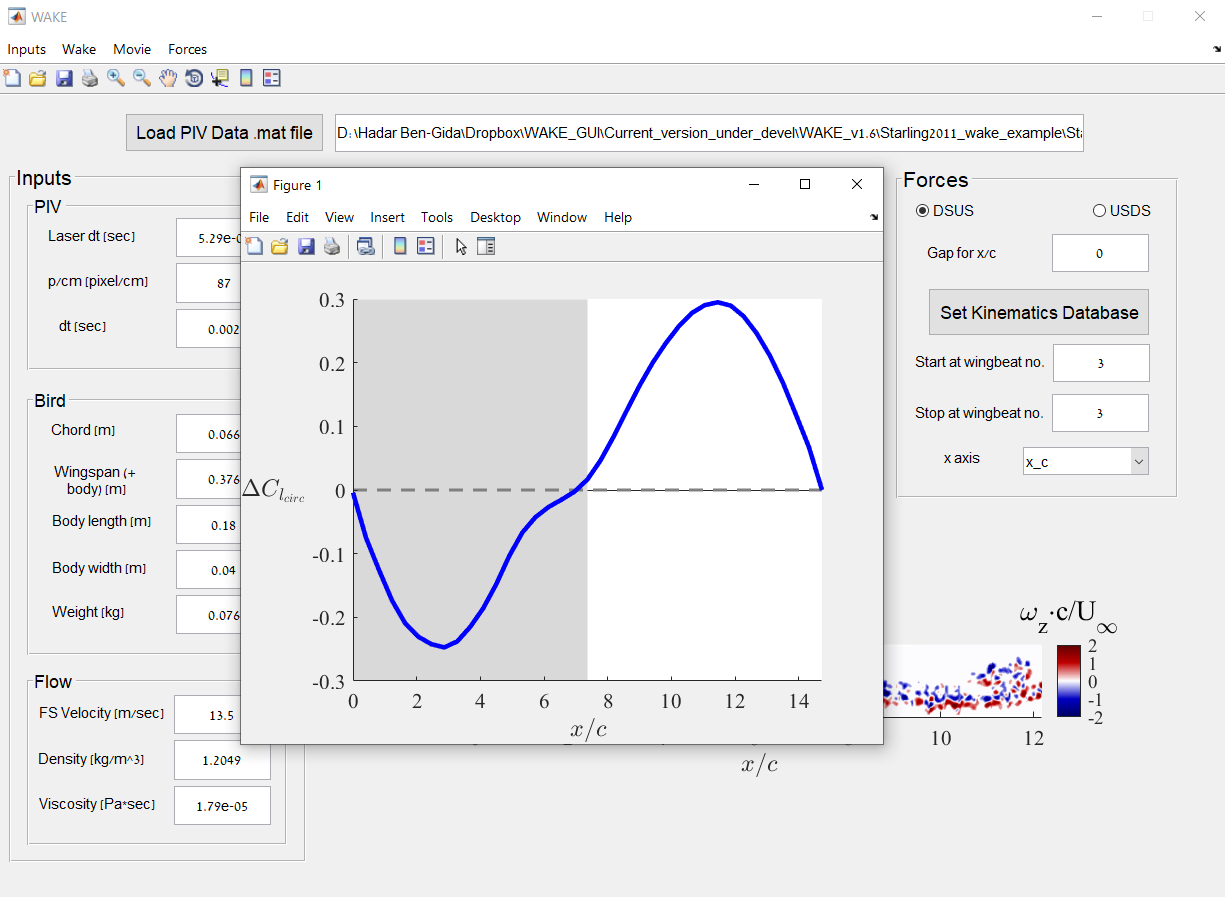
\includegraphics[width=0.79\textwidth]{dCl-plot-vs-x_c}
	\caption{Variation of the cumulative circulatory lift coefficient with $x/c$ for the $3^\mathrm{rd}$ Starling's wingbeat}
	\label{fig:GUI-dCl-plot-vs-x_c}
\end{figure}

\newpage
\begin{figure}[ht!]
	\centering
	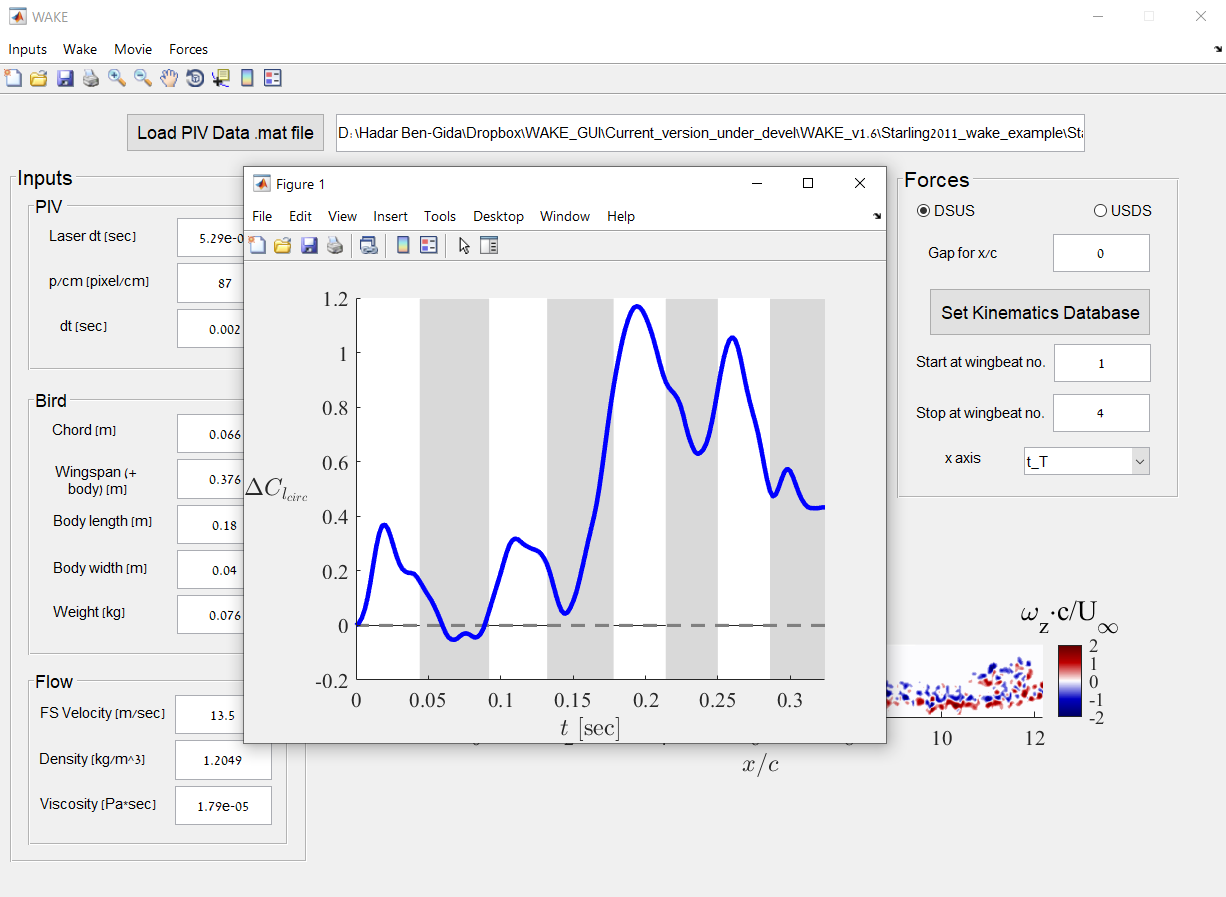
\includegraphics[width=0.8\textwidth]{dCl-plot-vs-time-4-wingbeats}
	\caption{Time variation of the cumulative circulatory lift coefficient for four consecutive Starling wingbeat}
	\label{fig:GUI-dCl-plot-vs-time-4-wingbeats}
\end{figure}

\begin{figure}[ht!]
	\centering
	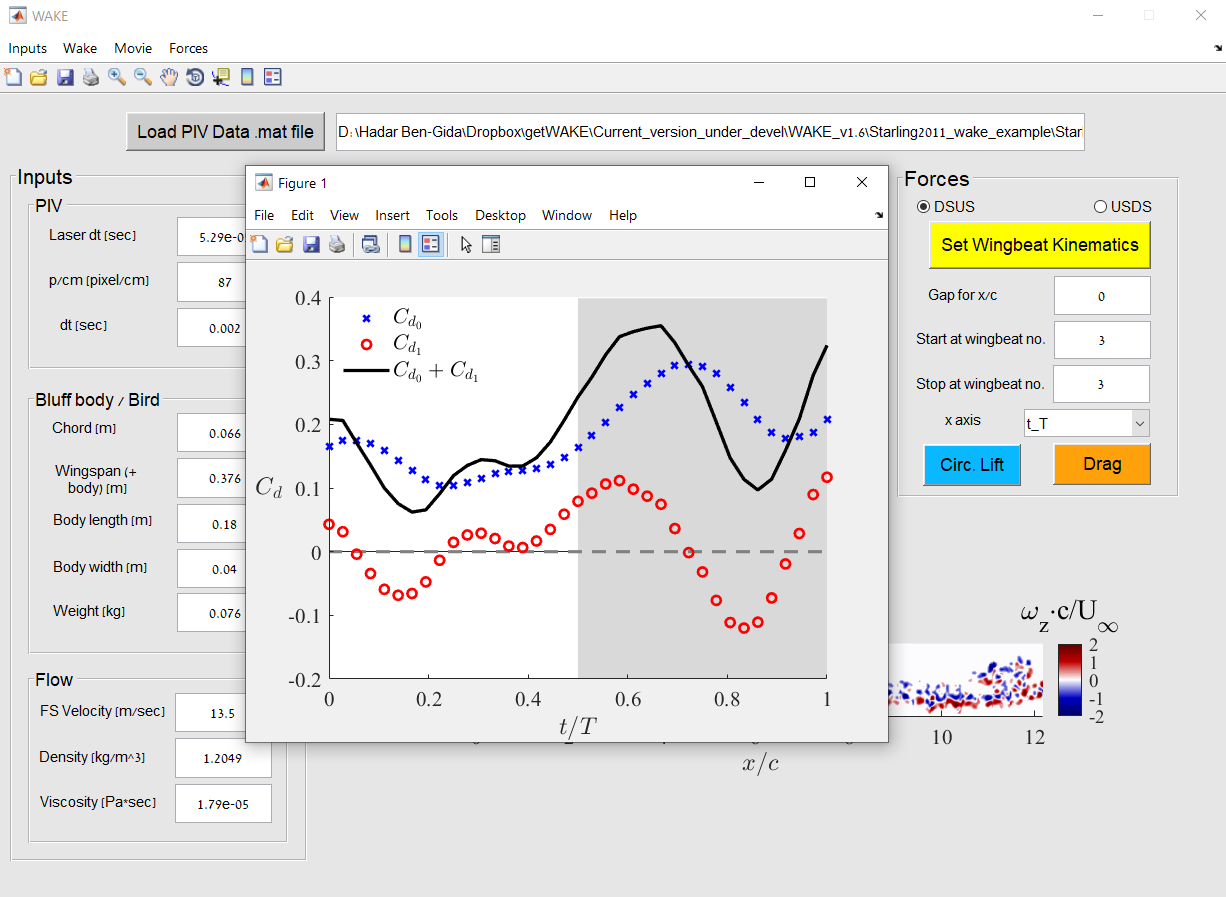
\includegraphics[width=0.8\textwidth]{drag-plot}
	\caption{Variation of the drag coefficient with $t/T$ for the $3^\mathrm{rd}$ Starling's wingbeat}
	\label{fig:GUI-drag-plot}
\end{figure}

\newpage
The method for computing the cumulative circulatory lift throughout the wake can be determined from the ``Define lift computation Method'' option under the drop-down menu ``Forces''. 
Either this option or its shortcut Ctrl+1 will open a new window entitled ``Movie properties'' (see \Cref{fig:GUI-Lift-comp-methods}), in which the user can set the method for computing the lift. A total of four options are available (\textit{default} method is ``\textit{Panda \& Zaman (1994), based on PIV individual maps (threshold applied)''}):
\begin{itemize}
	\item \textbf{Panda \& Zaman (1994), based on PIV individual maps (threshold applied)}: computing the cumulative circulatory lift coefficient, based on Panda and Zaman \cite{Panda1994}, from individual PIV maps data across the wake (after applying the threshold).
	\item \textbf{Panda \& Zaman (1994), based on generated wake}: computing the cumulative circulatory lift coefficient, based on Panda and Zaman \cite{Panda1994}, from the complete wake image data.
	\item \textbf{Panda \& Zaman (1994), based on generated wake (threshold applied)}: computing the cumulative circulatory lift coefficient, based on Panda and Zaman \cite{Panda1994}, from the complete wake image data (after applying the threshold).
	\item \textbf{Cumulative sum}: computing the cumulative circulatory lift coefficient from a direct summation of the circulation values of individual PIV maps along the wake (with the threshold applied).   
\end{itemize}
For more information regarding the above options, see \Cref{dCl_calc}. Further information regarding the drag coefficient computation is given in \Cref{Cd_calc}.

\begin{figure}[ht!]
	\centering
	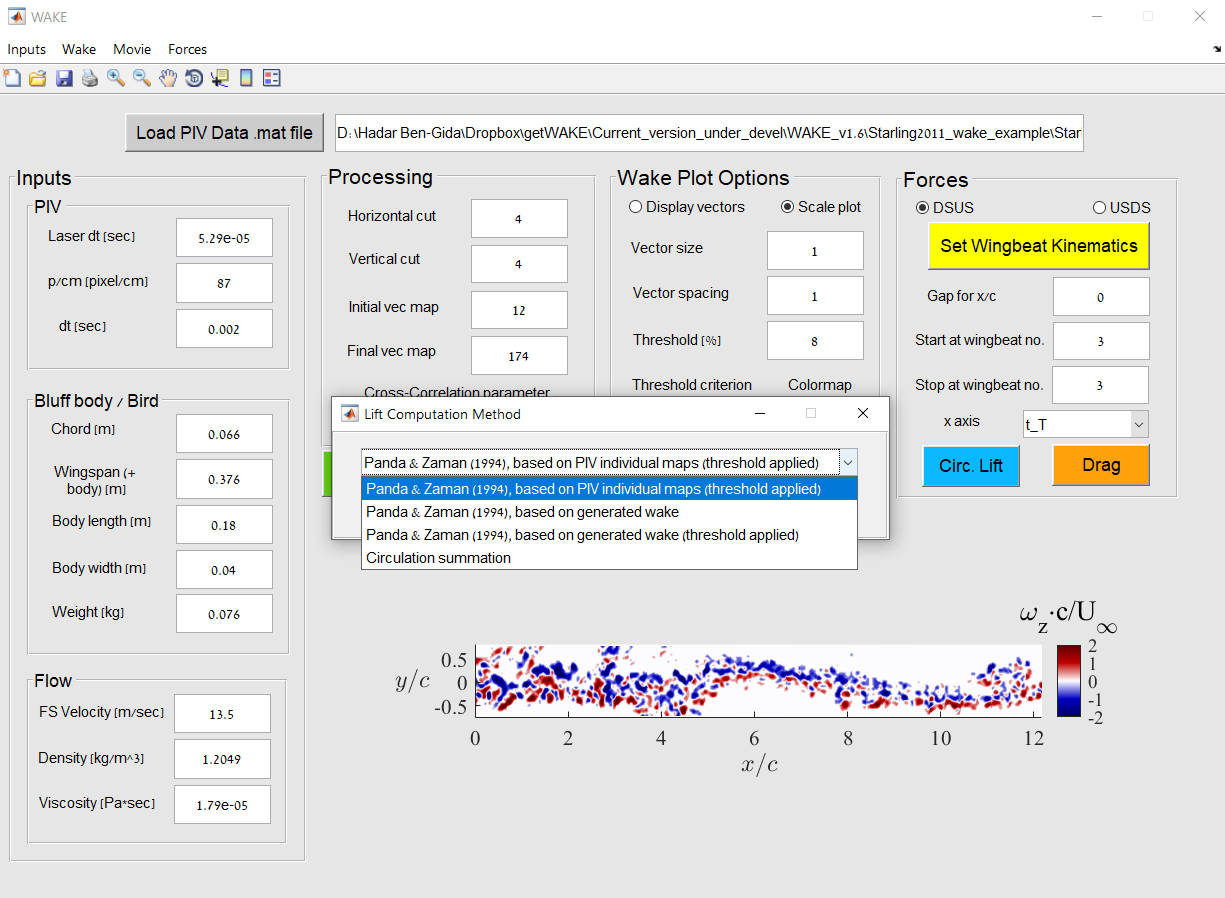
\includegraphics[width=0.85\textwidth]{Lift-comp-methods}
	\caption{Cumulative circulatory lift computation methods}
	\label{fig:GUI-Lift-comp-methods}
\end{figure}


\section{Wake Reconstruction}
The main motivation in the \emph{WAKE-GUI} Matlab Toolbox is to describe, visually, the wake evolution behind flapping birds or bodies undergoing unsteady motion to observe the formation of flow features as they shed downstream \cite{Ben-Gida2013,Nafi2020,Stalnov2015,Gurka2017,Lawley2019}. 
A detailed wake characterization can explain many of the phenomena that the source experienced. 
Utilization of a long-duration time-resolved PIV system enables the wake measurement behind birds' and moving bodies for a relatively long time (or distance) and with high spatial and temporal resolution. 
The wake reconstruction (see an example wake measured behind a flapping Starling in \Cref{fig:GUI-wake-evolution-example}), which is the main output of this toolbox, is based on PIV images taken from a stationary camera yielding Eulerian observation of the flow field behind the source. 
For the wake reconstruction, we assume the bird's/body's position did not change much relative to the measurement plane. 
Thus, invoking Taylor's hypothesis \cite{Taylor1938} allows the assumption that the flow remains relatively unchanged as it passes through the measurement plane. This hypothesis implies that there is no significant time dependence of a spatial velocity distribution over the timescale required for observation. 
Zaman and Hussain \cite{Zaman1981} showed that the hypothesis works well for an isolated coherent structure if a constant convection velocity, equal to the structure centre velocity, is used in the case of shear flows. 

The wake composite image is generated by offsetting each consecutive PIV image with a calculated instantaneous convection velocity and then overlapping the images, while keeping the mid region of each instantaneous PIV image. 
The instantaneous convection velocity, which determines the offset if each PIV image, is calculated based on a cross-correlation algorithm that examine the match of the velocity vector fields ($u,v$) or the fluctuating velocity vector fields ($u^{\prime},v^{\prime}$) of two consecutive PIV maps.
The cross-correlation coefficient, which determines the match of two consecutive PIV maps, is calculated as follows:
\begin{equation}
\begin{aligned}[b]
C_p(X,Y,T)&=    \\
&\sum_{i=1,j=1}^{I,J} \frac{\left[ p(x_i,y_i,t) - \overline{p(t)} \right] \left[ p(x_i+X,y_i+Y,t+T) - \overline{p(t+T)} \right]}{IJ\sigma_p(t)\sigma_p(t+T)}
\label{eq:Cp}
\end{aligned}
\end{equation}
If $C=1$, the two PIV maps are identical; i.e., perfectly matched. If the two images are different, then $C<1$.
$I,J$ is the size of the overlapping area and $\sigma_p$ is the standard deviation of the flow property $p$. Here, $p$ is to be replaced with $u$ and $v$ for computing the cross-correlation coefficients with respect to the velocity vector maps ($C_u,C_v$), or with $u^{\prime}$ and $v^{\prime}$ for computing the cross-correlation coefficients with respect to the velocity fluctuations vector maps ($C_{u^{\prime}},C_{v^{\prime}}$).
The spatial shift ($X,Y$) of any instantaneous PIV map is computed based on overlapping that achieves the maximum correlation coefficient; i.e., $\mathrm{max}\left[C_u,C_v\right]$ or $\mathrm{max}\left[C_{u^\prime},C_{v^\prime}\right]$.
If the cross-correlation failed during the \emph{WAKE-GUI} wake reconstruction process (e.g., due to poor PIV data), the spatial shift of each instantaneous PIV map is determined from the freestream advection velocity $U_\infty$ and the time difference $\Delta t$; i.e., $X=U_\infty\Delta t$.
Please note to not remove to many vector rows/columns from the PIV map (using ``Horizontal cut'' or ``Vertical cut''), otherwise the cross-correlation may fail due to insufficient overlapping area.

In the example wake below the bird flew from right to left; therefore, the downstream distance is measured as positive chord lengths. What appears as downstream essentially happened earlier, while what appears as upstream happened later. 
\begin{figure}[ht!]
	\centering
	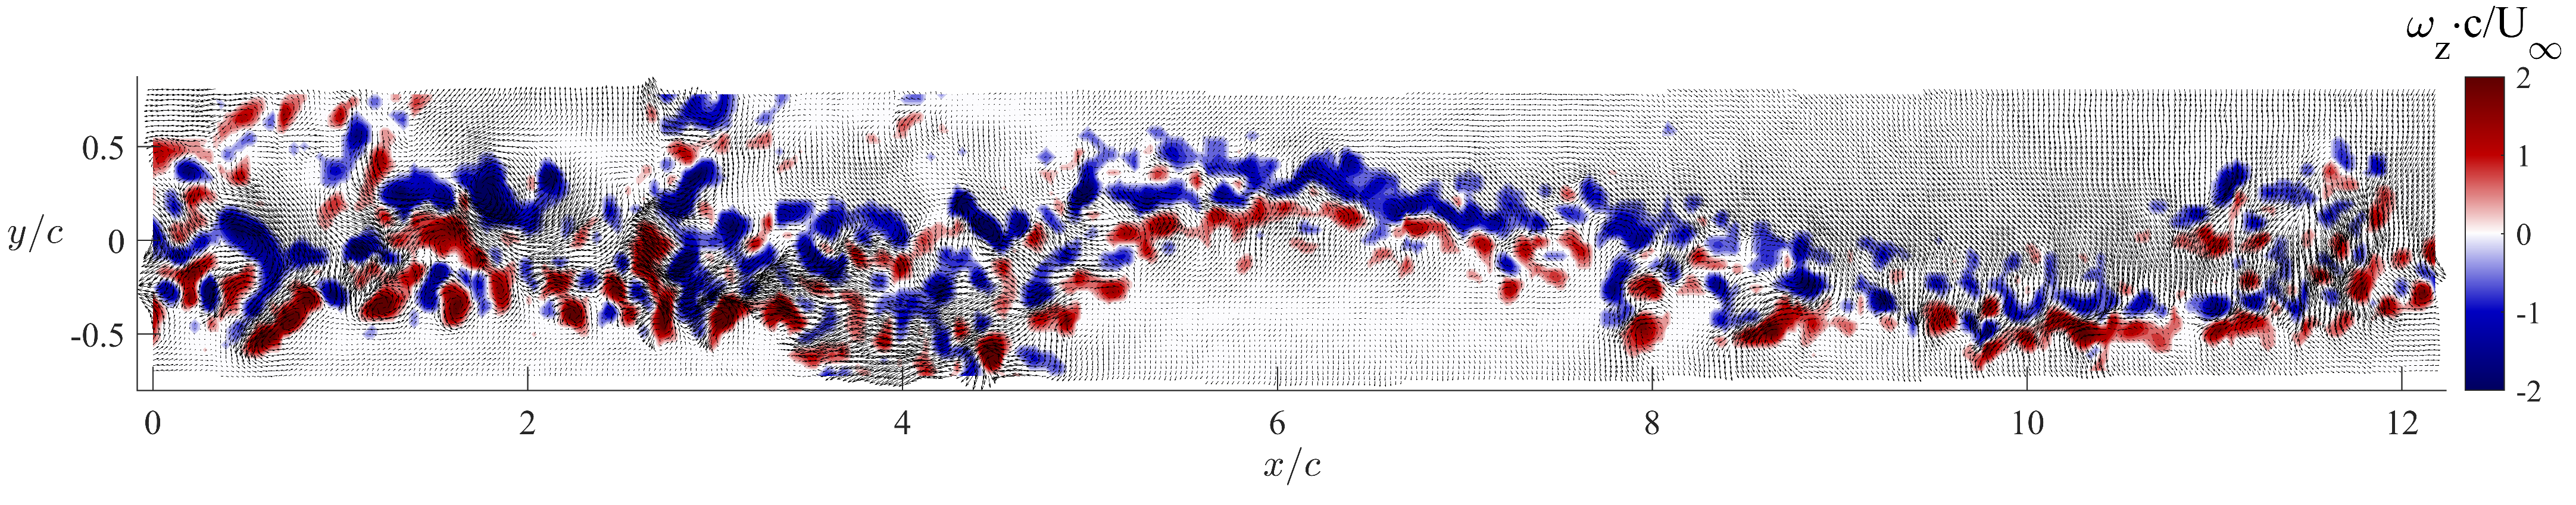
\includegraphics[width=\textwidth]{wake-evolution-example}
	\caption{Example of a wake reconstructed by the \emph{WAKE-GUI} from PIV wake measurements taken behind a freely flying Starling during a complete wingbeat. The contour is the normalized spanwise vorticity in the wake}
	\label{fig:GUI-wake-evolution-example}
\end{figure}


\section{Forces Estimation}\label{forces}
\subsection{Drag coefficient $C_d$}\label{Cd_calc}
The variation of the drag force can be estimated from the PIV wake data based on Ben-Gida et al. \cite{Ben-Gida2013}. 
The analysis leads to the following equation for the two-dimensional drag coefficient computed in the wake:
\begin{equation}
C_d = \underbrace{\frac{2}{cU_\infty}\int_0^h u\left(1 - \frac{u}{U_\infty}\right) \mathrm{d}y}_{C_{d_0}\text{ - Steady part}} - \underbrace{ \frac{2}{cU_\infty}\frac{\partial}{\partial t}\int_0^h \int_0^l \frac{u}{U_\infty} \mathrm{d}x\mathrm{d}y}_{C_{d_1}\text{ - Unsteady part}}
\label{eq:Cd}
\end{equation}
The steady drag coefficient component $C_{d_0}$ is referred to as the velocity deficit drag, whereas the unsteady drag coefficient component $C_{d_1}$ is added due to the unsteady flow motion.
While the steady drag term can be obtained from the near wake velocity field, the unsteady drag term requires information regarding the entire control surface surrounding the source over time. 
We assume most of the unsteady disturbances generated by the unsteady motion are obtained from the velocity field at the near wake where both unsteady contribution and viscous effects have not dissipated yet.
Therefore, we approximate the full surface integral of the unsteady term to include only the velocity field obtained from the PIV experiments in the near wake behind the birds/bodies. Here, $U_\infty$ is the mean undisturbed streamwise velocity, and $h$ and $l$ are the vertical and horizontal extent of the computed velocity field in the wake, respectively.
For the steady drag coefficient, we average the various profiles along the streamwise extent of each PIV map, thus yielding a single $C_{d_0}$ value to represent each PIV map. 
\Cref{fig:GUI-drag-plot} depicts an example of the drag coefficient variation in the wake measured behind a freely flying Starling.

\newpage
\subsection{Cumulative circulatory lift coefficient $\Delta C_{l_{circ}}$}\label{dCl_calc}
The variation of the cumulative circulatory lift coefficient can be estimated from the PIV wake data based on Stalnov et al. \cite{Stalnov2015}, Ben-Gida et al. \cite{BenGida2016} and Nafi et al. \cite{Nafi2020}.
Any unsteady motion of a lifting surface is accompanied by shedding of vortices into the wake. Assuming potential flow, one can utilize the unsteady thin airfoil theory \cite{Theodorsen1935,Sears1938}, which assumes a planar wake evolution, to compute the time-dependent lift of a two-dimensional lifting surface.
Theodorsen \cite{Theodorsen1935} derived an expression for total time-dependent lift which is composed of non-circulatory and circulatory terms whereas Sears and von-K\'{a}rm\'{a}n \cite{Sears1938} unsteady lift derivation contains quasi-steady term (produced by instantaneous bound circulation), added mass term (generated by inertia of the fluid moving along with the lifting surface) and wake-induced lift term (produced by the wake vorticity). For simple harmonic motion, both methods provide similar expressions. 
The non-circulatory term from Theodorsen's \cite{Theodorsen1935} formulation is essentially the added mass term whereas the circulatory term is equivalent to sum of quasi-steady lift term and wake-induced lift term. 

In the near wake of flapping birds, we assume that the wake has not deformed yet and interactions between the vortices shed into the wake are not significant \cite{Stalnov2015}, thus allowing the use of the planar wake assumption and consequently the unsteady thin airfoil theory. 
Although general trends may be well described with the use of such theory, it is the small scales in the wake that are actually of interest. 
When analyzing these vortical structures in the near wake of flying birds, one can deduce a more suitable viscous-based method for the unsteady lift estimation. 
The estimation of increment in the time-dependent lift throughout the wake is evaluated here from the PIV velocity fields by utilizing Wu's viscous flow approach \cite{Wu1981}, which was later expressed by Panda and Zaman \cite{Panda1994}.
Assuming two-dimensional, incompressible flow and neglecting the added mass term, the time-dependent circulatory lift force can be expressed as \cite{Panda1994}:
\begin{equation}
L_{circ}(t) = \underbrace{\rho \frac{\mathrm{d}}{\mathrm{d}t}\iint_Ax\omega_z(t)\mathrm{d}x\mathrm{d}y}_{\text{x-moment of the vorticity field}} + \underbrace{\rho U_\infty \int_0^t \int_0^h\nu \left( \frac{\partial^2u(t)}{\partial x^2} + \frac{\partial^2u(t)}{\partial y^2} \right)\mathrm{d}y \mathrm{d}t}_{\text{Diffusion contribution}}
\label{eq:inst_Lift}
\end{equation}
where $x$ and $y$ are the Cartesian coordinates defining the wake flow plane, with $x$ axis in the freestream direction. In the above equation, the first integral from left is the first $x$-moment of the vorticity field ($A$) in the wake, with $\omega_z(t)$ as the instantaneous spanwise vorticity field ($=\partial v/\partial x - \partial u/\partial y$) that is evaluated directly from the PIV data using a least squares differentiation scheme. The second integral from left is the contribution from the viscous term (diffusion), with $\nu$ as the kinematic viscosity and $h$ denoting the vertical extent of the computed velocity field in the wake. This term may be negligible in the far wake, yet, here we take it into account for near-wake effects. $\rho$ is the fluid density.
Please note that in our notation in \Cref{eq:inst_Lift}, a minus sign is \textbf{not} placed ahead of the first integral from left. This is because in our analysis we define positive vorticity values in the wake region as counter-clockwise vortices, whereas Panda and Zaman \cite{Panda1994} defined them as clockwise vortices.

\newpage
Applying Taylor's hypothesis (as introduced above for the wake reconstruction), $\mathrm{d} x = U_\infty \mathrm{d}t$, one can transform the spatial derivative in the left-side integral of \Cref{eq:inst_Lift} into a temporal one. 
Moreover, by interchanging the left-side integral in \Cref{eq:inst_Lift} with the time derivative (using Leibniz integral rule), one can re-write \Cref{eq:inst_Lift} as follows:
\begin{equation}
L_{circ}(t) = \rho U_\infty \int_0^t \left[ \int_0^h u\omega_z(t)\mathrm{d}y +  \int_0^h\nu \left( \frac{\partial^2u(t)}{\partial x^2} + \frac{\partial^2u(t)}{\partial y^2} \right)\mathrm{d}y \right] \mathrm{d}t
\label{eq:inst_Lift2}
\end{equation}
Therefore, the change in the lift in time $\delta\tau$ can be expressed accordingly:
\begin{equation}
\delta L_{circ} = \rho U_\infty  \delta\Gamma
\label{eq:delL}
\end{equation}
where the corresponding change in the circulation $\delta \Gamma$ is given by:
\begin{equation}
\delta\Gamma =  \int_0^h u\omega_z(t)\mathrm{d}y +  \int_0^h\nu \left( \frac{\partial^2u(t)}{\partial x^2} + \frac{\partial^2u(t)}{\partial y^2} \right)\mathrm{d}y
\label{eq:delGamma}
\end{equation}

Since at the beginning of the unsteady motion the lift is unknown, we shall refer to the estimated lift component as an increment in the circulatory lift \cite{Stalnov2015,BenGida2016} that is generated from the beginning of the motion. 
Based on \Cref{eq:inst_Lift2}, the cumulative circulatory lift at time $t$, $\Delta L_{circ}(t)$, is computed accordingly:
\begin{equation}
\Delta L_{circ} (t)= \rho U_\infty \int_0^t \zeta(t)\mathrm{d}t = \rho U_\infty \Gamma(t)
\label{eq:dL-circ}
\end{equation}
with the vorticity flux term $\zeta(t)$ being expressed as follows:
\begin{equation}
\zeta(t) = \int_0^h u_c\omega_z(t)\mathrm{d}y +  \int_0^h\nu \left( \frac{\partial^2u(t)}{\partial x^2} + \frac{\partial^2u(t)}{\partial y^2} \right)\mathrm{d}y
\label{eq:zeta_vs_time}
\end{equation}
Here, $u_c$ is the convection velocity at which the characteristics of the wake collectively travel downstream.
The cumulative circulatory lift coefficient at time $t$ is expressed as:
\begin{equation}
\Delta C_{l_{circ}}(t) = \frac{2}{cU_\infty} \int_0^t \zeta(t)\mathrm{d}t = \frac{2\Gamma(t)}{cU_\infty}
\label{eq:dCl-circ}
\end{equation}

As discussed in \Cref{forces_estimation}, the \emph{WAKE-GUI} suggests four methods for computing the cumulative circulatory lift coefficient in the wake. 
In the \textit{default} option entitled \textbf{Panda \& Zaman (1994), based on PIV individual maps (threshold applied)}, the vorticity flux $\zeta(t)$ defined by \Cref{eq:zeta_vs_time} is estimated \textbf{for each individual PIV map obtained in the near wake} behind the source as function of time; after applying a threshold on the vorticity contours. 
For each PIV map (or time $t$), the convection velocity is defined as the mean streamwise velocity component along the $x$-direction, $u_c\approx\langle{u}\rangle_x(y)$, and the spanwise vorticity field is estimated as the local mean spanwise vorticity along the $x$-direction, $\omega_z(x,y,t)\approx\langle{\omega_z}\rangle_x(y,t)$. 
Moreover, for each PIV map, the second order derivatives of $u$ are computed using a least squares differentiation scheme and then approximated with their local mean value along the $x$-direction, $\partial^2u(x,y,t)/\partial x^2\approx\langle{\partial^2u/\partial x^2}\rangle_x(y,t)$ and $\partial^2u(x,y,t)/\partial y^2\approx\langle{\partial^2u/\partial y^2}\rangle_x(y,t)$.
All the above vectors, representing each instantaneous velocity map, are then integrated over the $y$-direction to yield the vorticity flux $\zeta(t)$, as presented in \Cref{eq:zeta_vs_time}, and the cumulative circulatory lift coefficient in the wake (see \Cref{eq:dCl-circ}).

In the option entitled \textbf{Panda \& Zaman (1994), based on generated wake (threshold applied)}, the vorticity flux $\zeta(t)$ defined by \Cref{eq:zeta_vs_time} is estimated from the \textbf{complete wake image reconstructed by the user} behind the source; after applying a threshold on the vorticity contours. 
For the complete reconstructed wake image, the convection velocity is approximated as the freestream velocity, $u_c\approx U_\infty$. The spanwise vorticity field array is taken directly from the complete reconstructed wake (after the threshold selected by the user is applied), $\omega_z(x,y)$, where $x$-direction and time $t$ are interchangeable by applying $\mathrm{d}t=U_\infty\mathrm{d}x$.
The second order derivatives of $u$ are computed using a least squares differentiation scheme directly from the complete reconstructed wake, $\partial^2u(x,y)/\partial x^2$ and $\partial^2u(x,y)/\partial y^2$, where $x$-direction and time $t$ are interchangeable by applying $\mathrm{d}t=U_\infty\mathrm{d}x$.
All the above arrays, representing the full reconstructed wake map, are then integrated over the $y$-direction (at each $x$ location) to yield the vorticity flux $\zeta(t)$, as presented in \Cref{eq:zeta_vs_time}, and the cumulative circulatory lift coefficient in the wake (see \Cref{eq:dCl-circ}).

The option entitled \textbf{Panda \& Zaman (1994), based on generated wake} is identical to the former one and based on the complete wake image reconstructed by the user, but without applying the threshold on the processed vorticity field. 

In the option entitled \textbf{Cumulative sum} the cumulative circulatory lift coefficient is estimated from the \textbf{individual PIV maps} accordingly:
\begin{equation}
\Delta C_{l_{circ}}(t) = \frac{2}{cU_\infty} \int_0^t \gamma(t)\mathrm{d}t = \frac{2\Gamma(t)}{cU_\infty}
\label{eq:dCl-circ_option4}
\end{equation}
where $\gamma(t)$ is the instantaneous circulation value calculated for each individual PIV map, as follows:
\begin{equation}
\gamma(t) = \int_0^l \int_0^h \omega_z(x,y,t)\mathrm{d}x\mathrm{d}y
\label{eq:gamma_option4}
\end{equation}
$h$ and $l$ are the vertical and horizontal extent of the PIV velocity field, respectively.

\clearpage


%---------- Bibliography ------------------------------------------------
\bibliographystyle{unsrt}       % this means that the order of references
% is dtermined by the order in which the
% \cite and \nocite commands appear
\bibliography{refrences}	      	% list here all the bibliographies that
%                           	% you need.


\end{document}
